\documentclass[11pt,a4paper]{report}

% ============================================================
% PACKAGES
% ============================================================
\usepackage[utf8]{inputenc}
\usepackage[T1]{fontenc}
\usepackage[english]{babel}
\usepackage{geometry}
\geometry{margin=2.5cm}
\usepackage{graphicx}
\usepackage{tikz}
\usetikzlibrary{shapes.geometric, arrows.meta, positioning, fit, backgrounds}
\usepackage{xcolor}
\usepackage{hyperref}
\usepackage{booktabs}
\usepackage{longtable}
\usepackage{array}
\usepackage{enumitem}
\usepackage{fancyhdr}
\usepackage{titlesec}
\usepackage{tcolorbox}
\usepackage{listings}
\usepackage{parskip}
\usepackage{fancyvrb}
\usepackage{tabularx}

% ============================================================
% COLORS
% ============================================================
\definecolor{stblue}{RGB}{0, 51, 153}
\definecolor{stgray}{RGB}{100, 100, 100}
\definecolor{stlight}{RGB}{230, 240, 255}
\definecolor{projectgreen}{RGB}{0, 128, 64}

% ============================================================
% HYPERREF SETUP
% ============================================================
\hypersetup{
    colorlinks=true,
    linkcolor=stblue,
    urlcolor=stblue,
    citecolor=stblue
}

% ============================================================
% HEADERS / FOOTERS
% ============================================================
\pagestyle{fancy}
\fancyhf{}
\fancyhead[L]{\footnotesize AI Fundamentals — Training Guide}
\fancyhead[R]{\footnotesize STMicroelectronics}
\fancyfoot[C]{\thepage}
\renewcommand{\headrulewidth}{0.4pt}

% ============================================================
% CUSTOM BOXES
% ============================================================
\newtcolorbox{projectbox}{
    colback=stlight,
    colframe=stblue,
    fonttitle=\bfseries,
    title={\small \textcolor{stblue}{In our project}},
    boxrule=0.5pt,
    arc=3pt,
    left=6pt, right=6pt, top=4pt, bottom=4pt
}

\newtcolorbox{analogybox}{
    colback=yellow!5,
    colframe=orange!60,
    fonttitle=\bfseries,
    title={\small Analogy},
    boxrule=0.5pt,
    arc=3pt,
    left=6pt, right=6pt, top=4pt, bottom=4pt
}

% ============================================================
% LISTINGS STYLE
% ============================================================
\lstset{
    basicstyle=\ttfamily\small,
    frame=single,
    backgroundcolor=\color{gray!5},
    breaklines=true,
    columns=fullflexible
}

% ============================================================
% TITLE FORMATTING
% ============================================================
\titleformat{\chapter}[display]
    {\normalfont\Huge\bfseries\color{stblue}}
    {\chaptertitlename\ \thechapter}{20pt}{\Huge}

% ============================================================
% DOCUMENT
% ============================================================
\begin{document}

% ============================================================
% TITLE PAGE
% ============================================================
\begin{titlepage}
\centering
\vspace*{3cm}
{\Huge\bfseries\color{stblue} AI Fundamentals\\[0.5cm]}
{\Large A practical guide to Artificial Intelligence concepts\\[1cm]}
{\normalsize Clear explanations \textbullet{} Visual examples \textbullet{} Real-world analogies\\[3cm]}
{\large\textbf{Abir GHARBI}\\[0.5cm]}
{\large STMicroelectronics — Support \& Maintenance Team — 2026\\[2cm]}
\vfill
\end{titlepage}

% ============================================================
% TABLE OF CONTENTS
% ============================================================
\tableofcontents
\newpage

% ============================================================
% CHAPTER 1 — WHAT IS AI
% ============================================================
\chapter{What is Artificial Intelligence?}

\section{The Simple Definition}

Artificial Intelligence (AI) is the science of building computer systems that can perform tasks normally requiring human intelligence: understanding language, recognizing images, making decisions, and learning from experience.

\begin{analogybox}
Think of AI as a very fast, very obedient assistant. It never gets tired, can read thousands of documents in seconds, remembers everything perfectly --- but has \textbf{zero} common sense and only does what it was trained to do. It's a powerful tool, not a thinking being.
\end{analogybox}

\section{AI is NOT Magic}

This is the most important point to start with. AI systems are \textbf{software} built on mathematics and statistics. They do not think, feel, or understand. They process data, find patterns, and produce outputs based on those patterns.

An AI system is only as good as:
\begin{itemize}
    \item The \textbf{data} it was trained on (garbage in = garbage out)
    \item The \textbf{algorithms} humans chose for it
    \item The \textbf{evaluation} humans apply to verify it works
\end{itemize}

\section{Types of AI}

\begin{table}[h]
\centering
\begin{tabularx}{\textwidth}{l X X}
\toprule
\textbf{Type} & \textbf{What it does} & \textbf{Exists today?} \\
\midrule
Narrow AI & One specific task, does it very well & Yes (all current AI) \\
General AI & Any intellectual task like a human & No --- does not exist yet \\
Super AI & Surpasses all human intelligence & Science fiction \\
\bottomrule
\end{tabularx}
\end{table}

\textbf{Every AI system you interact with today --- ChatGPT, Google Translate, Siri, our STM32 chatbot --- is Narrow AI.} It excels at one thing but cannot do everything.

\section{The AI Family Tree}

Understanding AI requires seeing how different fields fit together. Think of it as a set of Russian nesting dolls:

\begin{figure}[h]
\centering
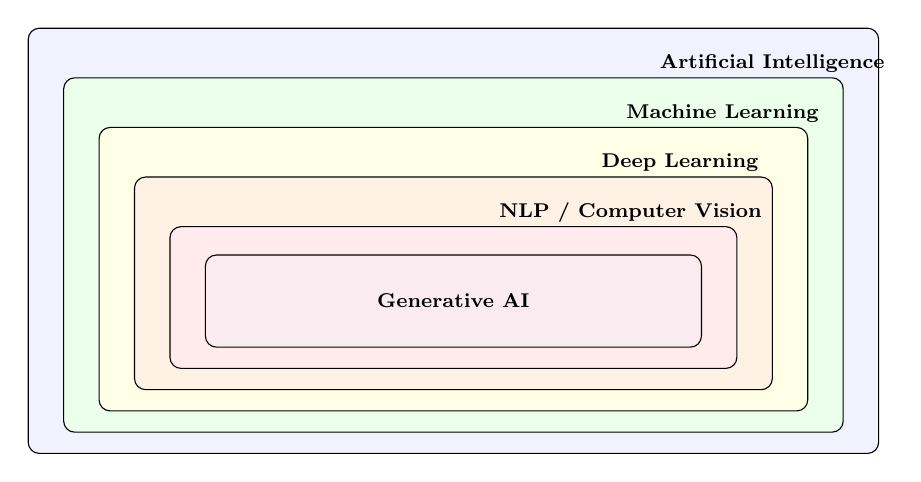
\begin{tikzpicture}[>=Stealth, scale=0.9, every node/.style={scale=0.9}]
  \draw[fill=blue!5, rounded corners] (0,0) rectangle (12,6);
  \node[font=\footnotesize] at (10.5,5.5) {\textbf{Artificial Intelligence}};
  \draw[fill=green!8, rounded corners] (0.5,0.3) rectangle (11.5,5.3);
  \node[font=\footnotesize] at (9.8,4.8) {\textbf{Machine Learning}};
  \draw[fill=yellow!10, rounded corners] (1,0.6) rectangle (11,4.6);
  \node[font=\footnotesize] at (9.2,4.1) {\textbf{Deep Learning}};
  \draw[fill=orange!10, rounded corners] (1.5,0.9) rectangle (10.5,3.9);
  \node[font=\footnotesize] at (8.5,3.4) {\textbf{NLP / Computer Vision}};
  \draw[fill=red!8, rounded corners] (2,1.2) rectangle (10,3.2);
  \node[font=\footnotesize] at (6,2.2) {\textbf{Large Language Models (GPT, Claude...)}};
  \draw[fill=purple!8, rounded corners] (2.5,1.5) rectangle (9.5,2.8);
  \node[font=\footnotesize] at (6,2.15) {\textbf{Generative AI}};
\end{tikzpicture}
\caption{The AI family tree: each layer is a specialization of the previous one.}
\label{fig:ai-family}
\end{figure}

The rest of this document follows this nesting: we start from the outside (AI, ML) and dive deeper until we reach Generative AI and LLMs.

% ============================================================
% CHAPTER 2 — MACHINE LEARNING
% ============================================================
\chapter{Machine Learning --- When Computers Learn from Data}

\section{The Fundamental Idea}

Machine Learning (ML) is where the story really begins. It is the subset of AI where systems \textbf{learn from data} instead of being explicitly programmed with rules.

\begin{table}[h]
\centering
\begin{tabularx}{\textwidth}{X X}
\toprule
\textbf{Traditional programming} & \textbf{Machine Learning} \\
\midrule
Human writes the rules & System discovers the rules \\
``IF email contains `free money' THEN spam'' & Show 10,000 labeled emails, system learns what spam looks like \\
Rules are brittle --- break on new patterns & Adapts to new patterns automatically \\
\bottomrule
\end{tabularx}
\end{table}

\begin{analogybox}
\textbf{The child learning fruits.} A child doesn't need a rulebook that says ``a fruit is round, colorful, grows on trees.'' Instead, you show the child 100 fruits and say ``this is an apple, this is a banana, this is a grape.'' After enough examples, the child recognizes new fruits they've never seen before. \textbf{That's ML}: learning from examples, not from rules.
\end{analogybox}

\section{What Makes ML Different: Statistics + Adaptation}

At its core, ML is \textbf{applied statistics at scale}. The system:

\begin{enumerate}
    \item Looks at thousands of examples
    \item Finds \textbf{statistical patterns} (correlations, frequencies, clusters)
    \item Builds a \textbf{mathematical model} that captures those patterns
    \item Uses that model to make \textbf{predictions} on new, unseen data
\end{enumerate}

\textbf{The key word is ADAPTATION}: unlike a fixed program, an ML system \textbf{improves} when you give it more data. More examples = better pattern detection = better predictions.

\section{The Role of Dataset Size}

Dataset size matters enormously --- but differently depending on the problem:

\begin{table}[h]
\centering
\begin{tabularx}{\textwidth}{l X X}
\toprule
\textbf{Dataset size} & \textbf{What's possible} & \textbf{Limitations} \\
\midrule
$<$ 100 examples & Simple rules, basic statistics & Model cannot generalize \\
100 -- 10,000 & Traditional ML works well & Need careful feature engineering \\
10,000 -- 1M & Deep Learning becomes viable & Need significant compute \\
$>$ 1 Billion & Large Language Models & Need massive GPU clusters \\
\bottomrule
\end{tabularx}
\end{table}

\begin{analogybox}
\textbf{Learning to cook.} With 5 recipes, you can follow instructions. With 500 recipes, you start seeing patterns (``most Italian dishes use olive oil and garlic''). With 50,000 recipes from all cultures, you understand cooking deeply enough to \textit{invent} new dishes. Dataset size determines how deep the learning goes.
\end{analogybox}

\section{The Three Types of Machine Learning}

\subsection{Supervised Learning --- Learning with a Teacher}

The system learns from \textbf{labeled examples}: input/output pairs where a human has provided the ``correct answer.''

\begin{itemize}
    \item \textbf{Classification}: assign a category (spam vs.\ not spam, bug vs.\ feature request)
    \item \textbf{Regression}: predict a number (temperature tomorrow, house price)
\end{itemize}

\begin{analogybox}
Like a student with an answer key. They study 1,000 solved exercises, then take an exam with new exercises. The more solved exercises they studied, the better they'll do on the exam.
\end{analogybox}

\subsection{Unsupervised Learning --- Learning without Labels}

The system finds patterns in data \textbf{without being told what to look for}. Nobody provides correct answers.

\begin{itemize}
    \item \textbf{Clustering}: group similar items (``these 500 issues are about the same bug'')
    \item \textbf{Dimensionality reduction}: simplify complex data while keeping the important stuff
\end{itemize}

\begin{analogybox}
Like sorting a pile of 1,000 foreign-language books into groups. You don't understand the text, but you can group them by cover color, size, thickness, and font style. You've found structure without anyone telling you what the ``right'' groups are.
\end{analogybox}

\subsection{Reinforcement Learning --- Learning by Trial and Error}

The system learns by \textbf{experimenting}: it takes actions, receives rewards or penalties, and gradually learns which actions lead to good outcomes.

\begin{itemize}
    \item Used in: game AI (AlphaGo), robotics, self-driving cars
\end{itemize}

\begin{analogybox}
Like training a dog: reward for sitting, nothing for jumping. After 100 attempts, the dog always sits because it has learned which action gets treats.
\end{analogybox}

\section{ML Algorithms --- The Toolbox}

Different problems need different tools. Here's a simplified view:

\begin{table}[h]
\centering
\begin{tabularx}{\textwidth}{l X X}
\toprule
\textbf{Algorithm family} & \textbf{How it works (simplified)} & \textbf{Good for} \\
\midrule
Linear models & Draw a straight line between categories & Simple classification \\
Decision trees & Ask yes/no questions in sequence & Tabular data \\
Random forests & Many trees voting together & Most structured data problems \\
Neural networks & Layers of connected neurons & Complex patterns (language, images) \\
k-NN & ``Look at the k most similar examples'' & Recommendation, similarity \\
\bottomrule
\end{tabularx}
\end{table}

\textbf{The takeaway}: you don't need to know the math. Just understand that ML = showing examples to a statistical system that learns patterns and makes predictions. The choice of algorithm depends on the data and the problem.

% ============================================================
% CHAPTER 3 — DEEP LEARNING
% ============================================================
\chapter{Deep Learning \& Neural Networks --- ML Goes Deeper}

\section{From ML to Deep Learning: The Natural Next Step}

We just saw that Machine Learning finds patterns in data. But traditional ML has a limitation: for complex problems (understanding language, recognizing faces, generating images), \textbf{you need to manually engineer the right features}. Someone has to decide WHAT information is useful.

\textbf{Deep Learning removes this limitation.} It automatically discovers what features are important --- learning not just the patterns, but also \textbf{how to represent the data} in the first place.

\begin{analogybox}
\textbf{Traditional ML} = You tell an artist ``paint a sunset with orange, pink, and gold colors'' (you specify the features).

\textbf{Deep Learning} = You show an artist 10,000 sunset photos and say ``learn to paint sunsets.'' The artist figures out which colors, shapes, and compositions matter --- on their own.
\end{analogybox}

\section{What is a Neural Network?}

A neural network is inspired by the human brain (very loosely). It consists of layers of connected ``neurons'' that process information step by step.

\begin{figure}[h]
\centering
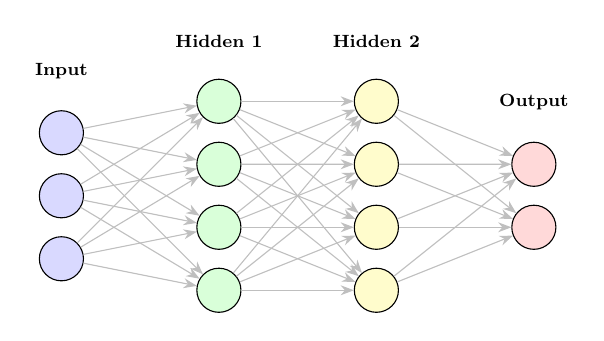
\begin{tikzpicture}[node distance=1.5cm, >=Stealth, scale=0.8, every node/.style={scale=0.8}]
  % Input layer
  \foreach \i in {1,2,3} {
    \node[circle, draw, fill=blue!15, minimum size=0.7cm] (i\i) at (0, -\i) {};
  }
  % Hidden layer 1
  \foreach \i in {1,2,3,4} {
    \node[circle, draw, fill=green!15, minimum size=0.7cm] (h1\i) at (2.5, -\i+0.5) {};
  }
  % Hidden layer 2
  \foreach \i in {1,2,3,4} {
    \node[circle, draw, fill=yellow!20, minimum size=0.7cm] (h2\i) at (5, -\i+0.5) {};
  }
  % Output layer
  \foreach \i in {1,2} {
    \node[circle, draw, fill=red!15, minimum size=0.7cm] (o\i) at (7.5, -\i-0.5) {};
  }
  % Connections
  \foreach \i in {1,2,3} {
    \foreach \j in {1,2,3,4} {
      \draw[->, gray!50] (i\i) -- (h1\j);
    }
  }
  \foreach \i in {1,2,3,4} {
    \foreach \j in {1,2,3,4} {
      \draw[->, gray!50] (h1\i) -- (h2\j);
    }
  }
  \foreach \i in {1,2,3,4} {
    \foreach \j in {1,2} {
      \draw[->, gray!50] (h2\i) -- (o\j);
    }
  }
  % Labels
  \node[above=0.3cm of i1, font=\footnotesize\bfseries] {Input};
  \node[above=0.3cm of h11, font=\footnotesize\bfseries] {Hidden 1};
  \node[above=0.3cm of h21, font=\footnotesize\bfseries] {Hidden 2};
  \node[above=0.3cm of o1, font=\footnotesize\bfseries] {Output};
\end{tikzpicture}
\caption{A neural network with 2 hidden layers. Each line is a ``weight'' --- a number adjusted during training.}
\label{fig:neural-network}
\end{figure}

\begin{itemize}
    \item \textbf{Input layer}: receives the raw data (text, image pixels, numbers)
    \item \textbf{Hidden layers}: progressively transform and abstract the data --- each layer detects increasingly complex patterns
    \item \textbf{Output layer}: produces the final result (a classification, a prediction, a generated word)
\end{itemize}

Each connection between neurons has a \textbf{weight} --- a number that gets adjusted during training. Training a neural network = finding the millions of weights that produce correct outputs.

\section{What Makes it ``Deep''?}

``Deep'' simply means \textbf{many layers}. A network with 2 layers is ``shallow.'' A network with 100+ layers is ``deep.'' More layers = the ability to learn more complex, abstract patterns.

\begin{table}[h]
\centering
\begin{tabularx}{\textwidth}{l c X}
\toprule
\textbf{Type} & \textbf{Layers} & \textbf{Capable of} \\
\midrule
Traditional ML & 0 (no layers) & Simple patterns, needs hand-crafted features \\
Shallow network & 1--3 layers & Basic pattern recognition \\
Deep network & 10--100+ & Language understanding, image recognition \\
Very deep (GPT-4) & 120+ layers & Complex reasoning, generation, translation \\
\bottomrule
\end{tabularx}
\end{table}

\section{Why Deep Learning Exploded in 2012}

Deep Learning concepts existed since the 1980s. So why did they only become powerful recently? Three things came together:

\begin{enumerate}
    \item \textbf{Massive data} --- the internet produced billions of texts, images, videos
    \item \textbf{Powerful GPUs} --- graphics cards designed for gaming turned out to be perfect for neural network math
    \item \textbf{Better algorithms} --- new training techniques (dropout, batch normalization, attention) that prevent the network from getting stuck
\end{enumerate}

\begin{analogybox}
Deep Learning is like a rocket engine that existed on paper for decades. It only flew when three things appeared simultaneously: enough fuel (data), a powerful enough engine (GPUs), and better aerodynamics (algorithms). Without all three, the rocket stays on the ground.
\end{analogybox}

\section{What Deep Learning Made Possible}

\begin{itemize}
    \item \textbf{Language understanding} --- chatbots, translation, summarization (→ leads to NLP and LLMs)
    \item \textbf{Image recognition} --- face unlock, medical imaging, autonomous driving
    \item \textbf{Speech recognition} --- Siri, Alexa, Google Assistant
    \item \textbf{Content generation} --- writing text, creating images, composing music
\end{itemize}

\textbf{The next chapter shows what happened when Deep Learning was applied specifically to language...}

% ============================================================
% CHAPTER 4 — HOW TO TRAIN A MODEL
% ============================================================
\chapter{How to Train a Model --- The Mechanics}

\section{The Big Picture: What Does ``Training'' Mean?}

Now that you understand what ML and neural networks are, let's look at \textbf{how} they actually learn.

When we say ``training a model,'' we mean: \textbf{showing it thousands of examples so it discovers the patterns by itself.}

The model starts knowing \textbf{nothing}. Through training, it gradually learns what matters and what doesn't.

\begin{analogybox}
\textbf{Learning to recognize cats.} Show a child 10,000 photos: some with cats, some without. At first, the child guesses randomly. But after thousands of examples with the label ``cat'' or ``not cat,'' the child notices: pointed ears, whiskers, fur, small nose... The child \textit{discovered} the rules from examples --- nobody listed them. \textbf{That's exactly how training works.}
\end{analogybox}

\section{The Training Lifecycle}

Training is not a single action --- it's a \textbf{cycle}. If one step is weak, everything suffers.

\begin{figure}[h]
\centering
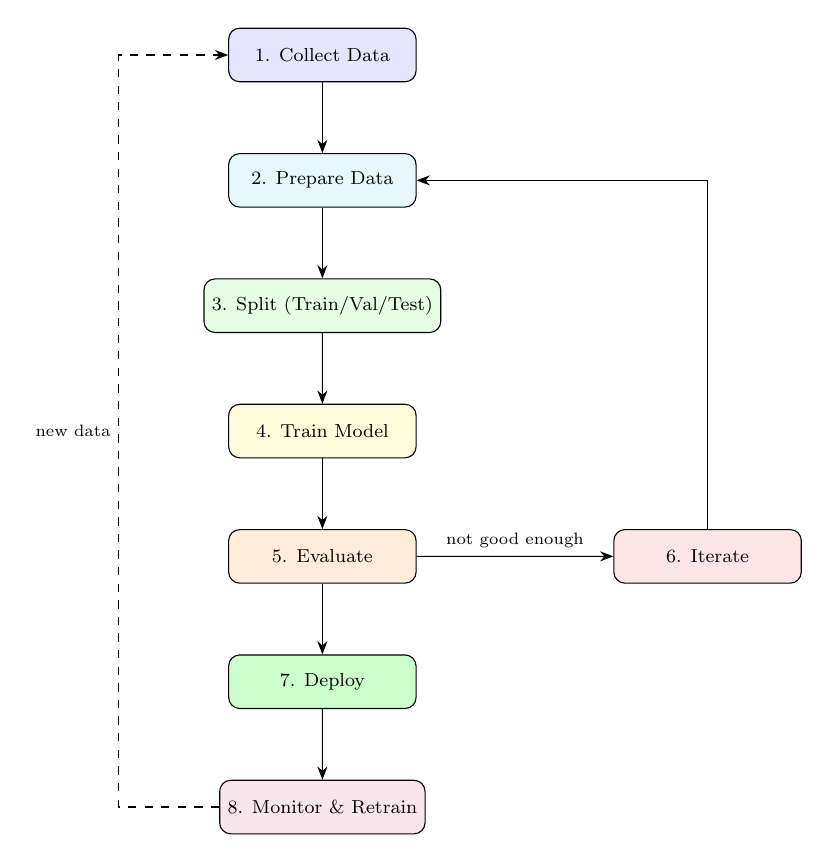
\begin{tikzpicture}[node distance=0.9cm, >=Stealth, scale=0.85, every node/.style={scale=0.85},
  step/.style={rectangle, rounded corners, draw, fill=#1, minimum height=0.8cm, minimum width=2.8cm, align=center, font=\footnotesize},
  step/.default=blue!10]
  \node[step=blue!10] (collect) {1. Collect Data};
  \node[step=cyan!10, below=of collect] (prepare) {2. Prepare Data};
  \node[step=green!10, below=of prepare] (split) {3. Split (Train/Val/Test)};
  \node[step=yellow!15, below=of split] (train) {4. Train Model};
  \node[step=orange!15, below=of train] (eval) {5. Evaluate};
  \node[step=red!10, right=2.5cm of eval] (iterate) {6. Iterate};
  \node[step=green!20, below=of eval] (deploy) {7. Deploy};
  \node[step=purple!10, below=of deploy] (monitor) {8. Monitor \& Retrain};
  \draw[->] (collect) -- (prepare);
  \draw[->] (prepare) -- (split);
  \draw[->] (split) -- (train);
  \draw[->] (train) -- (eval);
  \draw[->] (eval) -- (deploy);
  \draw[->] (deploy) -- (monitor);
  \draw[->] (eval) -- node[above, font=\scriptsize]{not good enough} (iterate);
  \draw[->] (iterate.north) |- (prepare.east);
  \draw[->, dashed] (monitor.west) -- ++(-1.5,0) |- node[left, pos=0.25, font=\scriptsize]{new data} (collect.west);
\end{tikzpicture}
\caption{The model training lifecycle: an iterative process with feedback loops.}
\label{fig:training-lifecycle}
\end{figure}

\subsection{Step 1: Collect Data}

You need \textbf{examples} of the problem you want to solve. More examples, and more diverse examples = better learning.

\textbf{Critical rule}: examples must be \textbf{representative} of real-world situations. Training only on English emails? The model will fail on French emails.

\subsection{Step 2: Prepare Data}

Raw data is never ready. You must:
\begin{enumerate}
    \item \textbf{Clean}: remove noise, fix errors, normalize formats
    \item \textbf{Engineer features}: extract the useful signals (more in Chapter~12)
    \item \textbf{Label}: tag each example with the correct answer
\end{enumerate}

\begin{analogybox}
\textbf{Kitchen prep.} Before cooking, you wash vegetables, peel them, cut them to size, remove bad parts. Data preparation is the kitchen prep of AI --- skip it, and the dish tastes terrible no matter how good the recipe.
\end{analogybox}

\subsection{Step 3: Split Data into Three Sets}

\begin{table}[h]
\centering
\begin{tabularx}{\textwidth}{l l X}
\toprule
\textbf{Set} & \textbf{Size} & \textbf{Purpose} \\
\midrule
Training set & $\sim$80\% & Model \textbf{learns} from these \\
Validation set & $\sim$10\% & Check progress \textbf{during} training \\
Test set & $\sim$10\% & Final measurement --- used \textbf{once} \\
\bottomrule
\end{tabularx}
\end{table}

\textbf{Why?} If you test on the same data you trained on, it's like a student who memorizes exact exam questions --- they'll score 100\% but fail any new question.

\begin{analogybox}
\textbf{Driving school.} Training set = practice drives. Validation set = mock exams. Test set = the real driving test on a route you've never driven. Pass that, and you can truly drive.
\end{analogybox}

\subsection{Step 4: Train the Model}

The actual learning happens in a loop:

\begin{enumerate}
    \item Take one example
    \item Make a prediction (initially random)
    \item Compare to the correct answer
    \item Calculate the \textbf{error} (how far off)
    \item Adjust internal weights slightly to reduce that error
    \item Repeat thousands/millions of times
\end{enumerate}

One full pass through all training data = one \textbf{epoch}. Models train for 10 to 1,000+ epochs.

\begin{analogybox}
\textbf{Darts.} First throw misses entirely. Feedback: ``too far left.'' Adjust. Next: ``a bit high.'' Adjust. After 1,000 throws, you consistently hit near the bullseye. Each throw = one training step. Feedback = the error. Your muscle adjustment = the weight update.
\end{analogybox}

\subsection{Step 5: Evaluate}

Measure performance on data the model has \textbf{never seen}:
\begin{itemize}
    \item \textbf{Accuracy}: \% of correct predictions
    \item \textbf{Precision}: when it says ``yes,'' how often is it right?
    \item \textbf{Recall}: of all actual positives, how many did it catch?
\end{itemize}

\subsection{Step 6: Iterate}

Not good enough? Don't throw everything away --- adjust:
\begin{itemize}
    \item More/better data → back to step 1
    \item Better features → back to step 2
    \item Different algorithm → change model
\end{itemize}

\subsection{Steps 7--8: Deploy \& Monitor}

Deploy to production. But models \textbf{degrade over time} (the world changes --- new patterns appear). This is \textbf{model drift}. Solution: retrain periodically with fresh data.

\section{What the Model Learns: Weights}

During training, the model adjusts millions of internal numbers called \textbf{weights}. GPT-4 has $\sim$1.8 \textbf{trillion} weights.

After training, weights are \textbf{frozen} --- the model stops learning and just applies what it knows.

\begin{analogybox}
\textbf{Mixing board.} A studio with 175 billion knobs. Training = turning every knob until the output sounds perfect. Once set, the studio produces great music for any song. The knob positions = the model's weights.
\end{analogybox}

\section{Overfitting vs.\ Underfitting}

\begin{table}[h]
\centering
\begin{tabularx}{\textwidth}{l X X}
\toprule
\textbf{Problem} & \textbf{What happens} & \textbf{Analogy} \\
\midrule
Overfitting & Memorizes training data, fails on new data & Student memorizes exact answers, can't solve variations \\
Underfitting & Too simple, misses patterns & Student didn't study enough, guesses randomly \\
Good fit & Learns patterns, generalizes well & Student understood concepts, solves new problems \\
\bottomrule
\end{tabularx}
\end{table}

\section{Training vs.\ RAG --- Two Different Approaches}

\begin{table}[h]
\centering
\begin{tabularx}{\textwidth}{l X X}
\toprule
& \textbf{Training a model} & \textbf{Using RAG} \\
\midrule
What you do & Teach the model (changes weights) & Give it documents to read at query time \\
Analogy & Teaching a language over months & Giving a dictionary to look up words \\
Time & Hours to weeks & Minutes to hours \\
Cost & Very expensive (GPU clusters) & Moderate \\
Updates & Retrain = slow \& expensive & Update docs = fast \& cheap \\
\bottomrule
\end{tabularx}
\end{table}

\begin{projectbox}
We don't train the LLM --- we optimize the DATA it retrieves. The LLM is a ``rented brain''; we make sure it has the right documents to read.
\end{projectbox}

% ============================================================
% CHAPTER 5 — NLP
% ============================================================
\chapter{Natural Language Processing --- Teaching Machines to Read}

\section{The Bridge: Deep Learning Meets Language}

We saw that Deep Learning excels at discovering patterns. When researchers applied DL to \textbf{text data}, an entire field was revolutionized: \textbf{Natural Language Processing} (NLP).

NLP is the branch of AI that enables computers to understand, interpret, and generate human language.

\begin{analogybox}
Imagine you land in a country where you don't speak the language. NLP is like a universal translator chip in your brain --- it converts any text or speech into something you understand, and lets you respond in that language. For computers, text is naturally a foreign language (they only understand numbers). NLP bridges that gap.
\end{analogybox}

\section{Why Language is Hard for Machines}

\begin{itemize}
    \item \textbf{Ambiguity}: ``bank'' = financial institution or river bank?
    \item \textbf{Context}: ``I saw her duck'' = she ducked, or she owns a duck?
    \item \textbf{Sarcasm/Irony}: ``Oh great, another meeting'' = not actually great
    \item \textbf{Coreference}: ``John told Peter that \textit{he} was wrong'' --- who is ``he''?
    \item \textbf{World knowledge}: understanding requires knowing things about the world
\end{itemize}

\section{Key NLP Tasks}

\begin{table}[h]
\centering
\begin{tabularx}{\textwidth}{l X X}
\toprule
\textbf{Task} & \textbf{What it does} & \textbf{Example} \\
\midrule
Tokenization & Split text into units & ``Hello world'' $\rightarrow$ [``Hello'', ``world''] \\
NER & Identify entities & ``STM32H7 has a bug'' $\rightarrow$ STM32H7=MCU \\
Sentiment Analysis & Detect emotion & ``Works perfectly!'' $\rightarrow$ positive \\
Classification & Assign categories & Email $\rightarrow$ spam / not spam \\
Summarization & Condense text & 10-page report $\rightarrow$ 3 sentences \\
Translation & Convert between languages & English $\rightarrow$ French \\
Question Answering & Extract answers & ``Capital of France?'' $\rightarrow$ ``Paris'' \\
\bottomrule
\end{tabularx}
\end{table}

\section{Tokenization: The First Step}

Before any NLP system can process text, the text must be split into smaller units called \textbf{tokens}. This is always step 1.

\begin{lstlisting}
"HAL_UART_Init() failed on STM32H7"
  -> ["HAL", "_", "UART", "_", "Init", "()", "failed", "on", "STM32", "H7"]
\end{lstlisting}

Modern LLMs use \textbf{subword tokenization} (BPE): common words stay whole, rare words are split into pieces. This way the model can handle any word --- even ones it has never seen.

\section{TF-IDF: Classic Word Importance}

Before Deep Learning dominated NLP, the standard technique was TF-IDF:

\begin{itemize}
    \item \textbf{TF} = how often a word appears in THIS document
    \item \textbf{IDF} = how rare the word is across ALL documents
    \item \textbf{TF-IDF = TF $\times$ IDF} = high score means the word is frequent here but rare elsewhere (= highly discriminating)
\end{itemize}

\textbf{Limitation}: TF-IDF treats words as independent units with no concept of meaning. ``UART error'' and ``USART failure'' would get zero similarity even though they mean the same thing. This is why embeddings (Chapter~9) replaced TF-IDF for semantic tasks.

\section{The Evolution of NLP}

\begin{table}[h]
\centering
\begin{tabularx}{\textwidth}{l l X}
\toprule
\textbf{Era} & \textbf{Period} & \textbf{Approach} \\
\midrule
Rule-based & 1950s--1990s & Hand-written grammar rules \\
Statistical & 1990s--2010s & Probabilities from large corpora (TF-IDF, n-grams) \\
Deep Learning & 2013--2017 & Neural networks (RNNs, LSTMs) \\
\textbf{Transformers} & \textbf{2017--now} & \textbf{Attention mechanism → GPT, BERT...} \\
\bottomrule
\end{tabularx}
\end{table}

The last row --- Transformers --- changed everything. That's the subject of the next chapter.

% ============================================================
% CHAPTER 6 — THE TRANSFORMER REVOLUTION
% ============================================================
\chapter{The Transformer Revolution --- How GPT Was Born}

\section{The Problem Before Transformers}

Before 2017, NLP models (RNNs, LSTMs) processed text \textbf{word by word, left to right}. This had two major problems:

\begin{enumerate}
    \item \textbf{Slow}: they couldn't process words in parallel --- each word had to wait for the previous one
    \item \textbf{Forgetful}: for long texts, the model ``forgot'' what was at the beginning by the time it reached the end
\end{enumerate}

\begin{analogybox}
Imagine reading a 500-page novel but you can only remember the last 50 pages. By the time you reach the ending, you've forgotten the beginning. Old NLP models had this exact problem with long texts.
\end{analogybox}

\section{The Breakthrough: Attention (2017)}

In 2017, researchers at Google published a paper titled \textit{``Attention Is All You Need.''} It introduced the \textbf{Transformer} architecture.

The key idea: \textbf{Attention} --- the model can look at ALL words in a text simultaneously and decide which ones are most relevant to each other.

\begin{itemize}
    \item Instead of reading left-to-right, the model sees the ENTIRE text at once
    \item For each word, it calculates how much ``attention'' to pay to every other word
    \item This allows understanding long-range relationships (``the cat that I saw yesterday at the park near the river'' --- ``cat'' connects to ``saw'' even though 8 words separate them)
\end{itemize}

\begin{analogybox}
\textbf{Old models} = reading a sentence with a tiny flashlight that only illuminates one word at a time.

\textbf{Transformers} = reading the entire page at once under full light, with the ability to draw arrows between related words no matter how far apart they are.
\end{analogybox}

\section{The Birth of GPT (2018)}

OpenAI took the Transformer architecture and asked: ``What if we train a massive Transformer on ALL the text on the internet, with one simple task: predict the next word?''

The result was \textbf{GPT} (Generative Pre-trained Transformer):
\begin{itemize}
    \item \textbf{Generative}: it generates text (predicts next word, again and again)
    \item \textbf{Pre-trained}: trained once on enormous data, then usable for many tasks
    \item \textbf{Transformer}: uses the attention mechanism
\end{itemize}

\section{The GPT Timeline --- A Story of Scale}

\begin{table}[h]
\centering
\begin{tabularx}{\textwidth}{l l X X}
\toprule
\textbf{Model} & \textbf{Year} & \textbf{Parameters} & \textbf{What changed} \\
\midrule
GPT-1 & 2018 & 117 million & Proof of concept: pre-training works \\
GPT-2 & 2019 & 1.5 billion & Writes coherent paragraphs --- OpenAI feared misuse \\
GPT-3 & 2020 & 175 billion & Few-shot learning: does tasks with just examples in prompt \\
GPT-4 & 2023 & $\sim$1.8 trillion & Near-human reasoning, multimodal (text + images) \\
\bottomrule
\end{tabularx}
\end{table}

\textbf{The pattern}: each generation was roughly 10$\times$ bigger. And each jump in scale produced \textbf{emergent abilities} --- capabilities that appeared ``spontaneously'' just from having more parameters and more data.

\begin{analogybox}
\textbf{GPT-2} (2019) was like a gifted student who can write decent essays.

\textbf{GPT-3} (2020) was like that student graduating university --- suddenly capable of translation, code, poetry, reasoning.

\textbf{GPT-4} (2023) is like that student becoming a polymath --- it handles text, images, logic, math, and code at near-expert level.

Each jump came not from teaching new tricks, but simply from \textit{making the model bigger and feeding it more data}.
\end{analogybox}

\section{Why ``Predict the Next Word'' is So Powerful}

This seems almost too simple. The model is just trained to predict what word comes next. But to predict well, the model must implicitly learn:

\begin{itemize}
    \item Grammar and syntax
    \item Facts about the world
    \item Logic and reasoning
    \item Cause and effect
    \item How to code, translate, summarize, answer questions...
\end{itemize}

All of this emerges from one objective: \textbf{predict the next token}. It's the simplest training objective that produces the most complex behavior.

\section{BERT vs.\ GPT --- Two Transformer Strategies}

\begin{table}[h]
\centering
\begin{tabularx}{\textwidth}{l X X}
\toprule
& \textbf{BERT (Google, 2018)} & \textbf{GPT (OpenAI, 2018+)} \\
\midrule
Direction & Reads text in both directions & Reads left-to-right only \\
Task & Fill in missing words (understanding) & Predict next word (generation) \\
Best for & Search, classification, Q\&A extraction & Text generation, chatbots, creation \\
Products & Google Search & ChatGPT, GitHub Copilot \\
\bottomrule
\end{tabularx}
\end{table}

% ============================================================
% CHAPTER 7 — GENERATIVE AI
% ============================================================
\chapter{Generative AI --- Machines That Create}

\section{What is Generative AI?}

Generative AI is the branch of AI that \textbf{creates new content} --- text, images, code, music, video --- that didn't exist before.

Before Generative AI, machines could only \textbf{analyze} (classify, detect, measure). Now they can \textbf{produce}:

\begin{table}[h]
\centering
\begin{tabularx}{\textwidth}{X X X}
\toprule
\textbf{Type of content} & \textbf{Tool} & \textbf{How it works} \\
\midrule
Text & ChatGPT, Claude, Gemini & Transformer predicts next word \\
Images & DALL-E, Midjourney, Stable Diffusion & Neural net generates pixels from description \\
Code & GitHub Copilot, Cursor & LLM trained on code repositories \\
Music & Suno, Udio & Neural net generates audio waveforms \\
Video & Sora, Runway & Frame-by-frame generation from text \\
\bottomrule
\end{tabularx}
\end{table}

\begin{analogybox}
\textbf{Traditional AI} = a camera (it captures and analyzes what exists).

\textbf{Generative AI} = a painter (it creates something new that never existed before).

Both are impressive, but only the painter produces original content.
\end{analogybox}

\section{How Generative AI Works (Simplified)}

All generative models follow the same fundamental pattern:

\begin{enumerate}
    \item \textbf{Learn the structure} of the training data (what a sentence looks like, what a face looks like, what code looks like)
    \item \textbf{Given a prompt} (instruction or starting point), generate new content that \textbf{follows the same structure}
    \item \textbf{Output} looks like it could be real --- but was created from scratch
\end{enumerate}

For text (GPT), this means: having seen trillions of words, the model knows what ``good text'' looks like. When you ask a question, it generates an answer word-by-word, each word chosen to be the most likely continuation.

\section{The Generative AI Ecosystem (2024--2026)}

\begin{table}[h]
\centering
\begin{tabularx}{\textwidth}{l l X}
\toprule
\textbf{Category} & \textbf{Key players} & \textbf{Our relevance} \\
\midrule
Foundation models & OpenAI, Anthropic, Google, Meta & We use Azure OpenAI (GPT) \\
Enterprise platforms & Microsoft (Azure), AWS (Bedrock) & ST ChatGPT runs on Azure \\
Coding assistants & GitHub Copilot, Cursor & Used for pipeline development \\
Image generation & DALL-E, Midjourney & Not used in our project \\
Specialized agents & Custom deployments & Our preprocessing agent \\
\bottomrule
\end{tabularx}
\end{table}

\section{Why Generative AI Changed Everything}

Before 2022, AI was mostly invisible to non-specialists. Since ChatGPT (November 2022), everyone can interact with AI directly. This changed:

\begin{itemize}
    \item \textbf{Accessibility}: anyone can use AI without coding
    \item \textbf{Productivity}: writing, coding, research became 2--10$\times$ faster
    \item \textbf{Expectations}: people now expect AI-powered features everywhere
    \item \textbf{Enterprise adoption}: companies rushed to integrate AI into workflows
\end{itemize}

\textbf{But generative AI has a critical weakness}: it can generate \textbf{confident nonsense} (hallucination). This is exactly why technologies like RAG (Chapter~11) exist --- to ground generative AI in verified facts.

% ============================================================
% CHAPTER 8 — LLMs AND THEIR ECOSYSTEM
% ============================================================
\chapter{Large Language Models --- The Engines of Modern AI}

\section{What is an LLM?}

A Large Language Model is a Deep Learning model (specifically a Transformer) trained on enormous amounts of text. It learns to predict what comes next, and from this develops the ability to understand and generate language.

\textbf{``Large''} refers to both:
\begin{itemize}
    \item The \textbf{model size}: billions to trillions of parameters (weights)
    \item The \textbf{training data}: trillions of words from books, websites, code, conversations
\end{itemize}

\begin{analogybox}
An LLM is like someone who has read every book, every website, and every forum in the world. They can talk about anything convincingly --- but they might mix things up or make things up, because they don't truly ``understand'' --- they just know what words typically follow other words.
\end{analogybox}

\section{How LLMs Generate Text}

LLMs produce text \textbf{one token at a time}. For each position, the model calculates the probability of every possible next word and picks one:

\begin{lstlisting}
Input:  "How do I initialize"   -> predicts: "UART"
Then:   "How do I initialize UART"   -> predicts: "on"
Then:   "How do I initialize UART on"   -> predicts: "STM32H7"
...continues until the answer is complete
\end{lstlisting}

The model never ``plans'' the full answer in advance. It generates word by word, always choosing the most probable continuation given everything that came before.

\section{The Hallucination Problem}

\textbf{The most dangerous weakness of LLMs}: they can generate information that sounds completely correct but is \textbf{entirely false}.

\begin{table}[h]
\centering
\begin{tabularx}{\textwidth}{X X}
\toprule
\textbf{Hallucination example} & \textbf{Why dangerous} \\
\midrule
``This bug was fixed in v1.4.2'' & Version might not exist --- wrong firmware choice \\
``Use HAL\_DMA\_Start\_IT() with channel 3'' & Wrong channel = potential hardware damage \\
``According to the datasheet, max clock is 200MHz'' & Wrong spec = design failure \\
\bottomrule
\end{tabularx}
\end{table}

\textbf{Why it happens}: the model generates the most \textit{statistically likely} continuation, not the most \textit{factually correct} one. It has no concept of truth --- only of probability.

\textbf{Solution}: RAG (Chapter~11) --- force the LLM to answer ONLY from retrieved, verified documents.

\section{Key LLM Concepts}

\begin{table}[h]
\centering
\begin{tabularx}{\textwidth}{l X}
\toprule
\textbf{Concept} & \textbf{What it means} \\
\midrule
Prompt & The text you send (question + context + instructions) \\
Context window & Max text the model can process at once (e.g.\ 128K tokens for GPT-4) \\
Temperature & Controls randomness: 0 = deterministic, 1 = creative \\
System prompt & Hidden instructions defining behavior (``You are a helpful STM32 expert...'') \\
Fine-tuning & Additional training on domain-specific data (expensive, permanent) \\
Tokens & Smallest text units (roughly: 1 token $\approx$ 0.75 words) \\
\bottomrule
\end{tabularx}
\end{table}

\section{The LLM Landscape (2024--2026)}

\begin{table}[h]
\centering
\begin{tabularx}{\textwidth}{l l X}
\toprule
\textbf{Model family} & \textbf{Company} & \textbf{Characteristics} \\
\midrule
GPT-4, GPT-4o & OpenAI & Most widely deployed, multimodal \\
Claude 3/4 & Anthropic & Strong reasoning, safety-focused \\
Gemini & Google & Integrated with Google ecosystem \\
LLaMA 3 & Meta & Open-weight, self-hostable \\
Mistral & Mistral AI (France) & Efficient, strong for its size \\
\bottomrule
\end{tabularx}
\end{table}

\section{LLM Limitations --- What They Cannot Do}

\begin{itemize}
    \item \textbf{No real-time knowledge}: training data has a cutoff date
    \item \textbf{No memory between conversations}: each chat starts fresh (unless engineered otherwise)
    \item \textbf{Cannot verify facts}: no access to ground truth during generation
    \item \textbf{Cannot reason reliably}: appears to reason but can make logical errors
    \item \textbf{Cannot learn from interaction}: weights are frozen after training
\end{itemize}

These limitations explain why \textbf{RAG, tools, and agents} are necessary: they compensate for what LLMs cannot do alone.

\begin{projectbox}
ST ChatGPT uses GPT (via Azure OpenAI) as its LLM. We don't train or fine-tune it --- we feed it the right documents through RAG, and define its behavior through a system prompt (persona).
\end{projectbox}

% ============================================================
% CHAPTER 9 — EMBEDDINGS
% ============================================================
\chapter{Embeddings --- How AI Understands Meaning}

\section{The Problem: Computers Only Understand Numbers}

Computers cannot read text the way we do. They need text converted into \textbf{numbers} --- but not random numbers. Numbers that capture the \textbf{meaning}.

\section{What is an Embedding?}

An embedding is a list of numbers (a vector) that represents the \textbf{meaning} of a piece of text. Texts with similar meanings get similar vectors.

``UART initialization error'' and ``USART init failure'' would have nearly identical embeddings because they mean the same thing --- even though they use completely different words.

\begin{analogybox}
Think of GPS coordinates. Paris and Lyon are both in France, so their coordinates are close together. Tokyo is far away, so its coordinates are very different. \textbf{Embeddings work the same way but for meaning}: similar texts are ``close'' in embedding space, unrelated texts are ``far apart.''
\end{analogybox}

\section{Why Embeddings Matter for Search}

\begin{table}[h]
\centering
\begin{tabularx}{\textwidth}{X X}
\toprule
\textbf{Keyword search (TF-IDF)} & \textbf{Semantic search (embeddings)} \\
\midrule
Matches exact words & Matches meaning \\
``UART error'' won't find ``USART failure'' & ``UART error'' WILL find ``USART failure'' \\
Simple but brittle & Robust to synonyms \\
\bottomrule
\end{tabularx}
\end{table}

\section{Cosine Similarity}

To measure how similar two embeddings are, we use \textbf{cosine similarity} --- a number between 0 (completely different) and 1 (identical meaning):

\begin{table}[h]
\centering
\begin{tabularx}{\textwidth}{X X c}
\toprule
\textbf{Text A} & \textbf{Text B} & \textbf{Similarity} \\
\midrule
UART init error on H7 & USART initialization failure STM32H7 & 0.92 \\
UART init error on H7 & How to configure SPI clock & 0.15 \\
\bottomrule
\end{tabularx}
\end{table}

\section{Embeddings Are the Foundation of RAG}

In a RAG system:
\begin{enumerate}
    \item All documents are converted to embeddings and stored in a vector database
    \item When a user asks a question, the question is also converted to an embedding
    \item The system finds documents whose embeddings are closest to the question's embedding
    \item Those documents are given to the LLM to generate the answer
\end{enumerate}

\textbf{Without good embeddings, RAG cannot work.} This is why data quality matters: garbage text produces garbage embeddings, which means wrong documents are retrieved.

% ============================================================
% CHAPTER 10 — SPECIALIZED CHATBOTS
% ============================================================
\chapter{Specialized Chatbots --- Why Generic AI Isn't Enough}

\section{Generalist vs.\ Specialized}

\begin{table}[h]
\centering
\begin{tabularx}{\textwidth}{l X X}
\toprule
& \textbf{Generalist (ChatGPT free)} & \textbf{Specialized (our chatbot)} \\
\midrule
Knowledge & Broad but shallow & Deep in one domain \\
Accuracy & Hallucination risk & Answers grounded in KB \\
Data source & The entire internet & Our curated documents \\
Updates & Waits for model retraining & KB updated anytime \\
\bottomrule
\end{tabularx}
\end{table}

\section{Why Specialize?}

A generalist LLM does \textbf{not} know:
\begin{itemize}
    \item The specific bugs of HAL STM32H7 v1.11.0
    \item The exact DMA configuration for an SPI transfer
    \item Workarounds validated by the firmware team
\end{itemize}

You must \textbf{provide this information at query time} → that's the role of RAG.

\section{Three Approaches to Specialization}

\begin{table}[h]
\centering
\begin{tabularx}{\textwidth}{l X X X}
\toprule
\textbf{Approach} & \textbf{How} & \textbf{Pros} & \textbf{Cons} \\
\midrule
Fine-tuning & Retrain on your data & Deeply integrated & Expensive, risks ``forgetting'' \\
RAG & Provide docs at query time & Flexible, traceable, updatable & Depends on retrieval quality \\
Prompt engineering & Detailed instructions & Quick to set up & Limited by context window \\
\bottomrule
\end{tabularx}
\end{table}

\section{Why We Chose RAG}

\begin{itemize}
    \item Data changes constantly (new issues, firmware releases)
    \item Every answer must cite its source (traceability)
    \item Fine-tuning would require expensive retraining at every update
    \item RAG: update the Knowledge Base in minutes, model stays the same
\end{itemize}

% ============================================================
% CHAPTER 11 — RAG
% ============================================================
\chapter{RAG --- Retrieval-Augmented Generation}

\section{The Problem RAG Solves}

Standard LLMs answer from their training data --- which is frozen, generic, and may be wrong for your specific domain.

\begin{table}[h]
\centering
\begin{tabularx}{\textwidth}{X X}
\toprule
\textbf{LLM alone} & \textbf{LLM + RAG} \\
\midrule
Answers from general training & Answers from YOUR documents \\
May be outdated & Uses your latest data \\
Cannot cite sources & Every answer traceable \\
High hallucination risk & Grounded in facts \\
\bottomrule
\end{tabularx}
\end{table}

\section{How RAG Works --- Step by Step}

\begin{enumerate}
    \item \textbf{User asks a question} --- ``How to configure DMA on STM32H7?''
    \item \textbf{RETRIEVAL} --- Search the Knowledge Base for the most similar documents (using embeddings)
    \item \textbf{Top-k documents retrieved} --- The most relevant chunks are selected
    \item \textbf{AUGMENTED GENERATION} --- LLM receives: question + retrieved docs
    \item \textbf{Answer generated} --- LLM synthesizes a precise, sourced answer
\end{enumerate}

\begin{figure}[h]
\centering
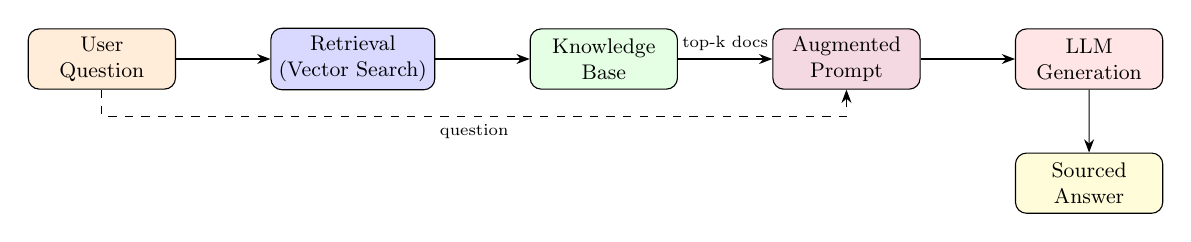
\begin{tikzpicture}[node distance=1.2cm, >=Stealth, scale=0.85, every node/.style={scale=0.85},
  box/.style={rectangle, rounded corners, draw, fill=#1, minimum height=0.9cm, minimum width=2.2cm, align=center, font=\small},
  box/.default=blue!10]
  \node[box=orange!15] (user) {User\\Question};
  \node[box=blue!15, right=of user] (retrieval) {Retrieval\\(Vector Search)};
  \node[box=green!10, right=of retrieval] (kb) {Knowledge\\Base};
  \node[box=purple!15, right=of kb] (augment) {Augmented\\Prompt};
  \node[box=red!10, right=of augment] (llm) {LLM\\Generation};
  \node[box=yellow!15, below=0.8cm of llm] (answer) {Sourced\\Answer};
  \draw[->] (user) -- (retrieval);
  \draw[->] (retrieval) -- (kb);
  \draw[->] (kb) -- node[above, font=\scriptsize]{top-k docs} (augment);
  \draw[->] (augment) -- (llm);
  \draw[->] (llm) -- (answer);
  \draw[->, dashed] (user.south) -- ++(0,-0.4) -| node[below, pos=0.25, font=\scriptsize]{question} (augment.south);
\end{tikzpicture}
\caption{RAG flow: Retrieval $\rightarrow$ Augmentation $\rightarrow$ Generation.}
\label{fig:rag-flow}
\end{figure}

\section{Why Data Quality is CRITICAL for RAG}

RAG can only work if:
\begin{enumerate}
    \item The \textbf{right data exists} in the KB (Data Generation)
    \item The data is \textbf{well structured} to be found (Feature Engineering + Chunking)
    \item The \textbf{retrieval works} (Similarity + Evaluation)
\end{enumerate}

$\rightarrow$ This is the role of our pipeline: transform raw data into optimized data so RAG works.

\begin{figure}[h]
\centering
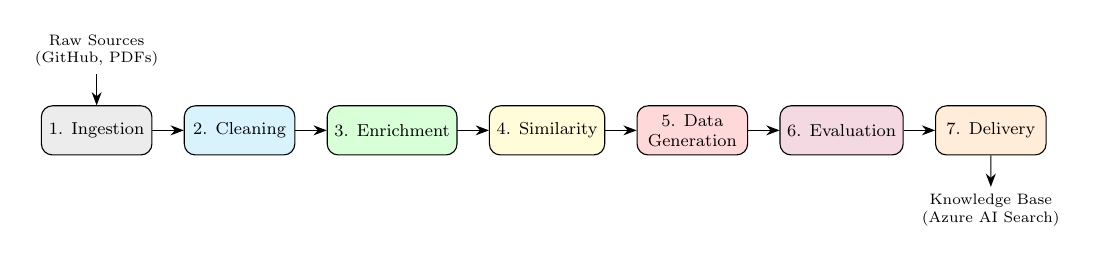
\begin{tikzpicture}[node distance=0.4cm, >=Stealth, scale=0.78, every node/.style={scale=0.78},
  stage/.style={rectangle, rounded corners, draw, fill=#1, minimum height=0.8cm, minimum width=1.8cm, align=center, font=\footnotesize},
  stage/.default=blue!10]
  \node[stage=gray!15] (ingest) {1. Ingestion};
  \node[stage=cyan!15, right=of ingest] (clean) {2. Cleaning};
  \node[stage=green!15, right=of clean] (enrich) {3. Enrichment};
  \node[stage=yellow!15, right=of enrich] (sim) {4. Similarity};
  \node[stage=red!15, right=of sim] (gen) {5. Data\\Generation};
  \node[stage=purple!15, right=of gen] (eval) {6. Evaluation};
  \node[stage=orange!15, right=of eval] (deliv) {7. Delivery};
  \draw[->] (ingest) -- (clean);
  \draw[->] (clean) -- (enrich);
  \draw[->] (enrich) -- (sim);
  \draw[->] (sim) -- (gen);
  \draw[->] (gen) -- (eval);
  \draw[->] (eval) -- (deliv);
  \node[above=0.4cm of ingest, font=\scriptsize, align=center] (src) {Raw Sources\\(GitHub, PDFs)};
  \draw[->] (src) -- (ingest);
  \node[below=0.4cm of deliv, font=\scriptsize, align=center] (kb) {Knowledge Base\\(Azure AI Search)};
  \draw[->] (deliv) -- (kb);
\end{tikzpicture}
\caption{Our preprocessing pipeline: 7 stages from raw data to RAG-ready Knowledge Base.}
\label{fig:pipeline-architecture}
\end{figure}

\section{Chunking Strategies}

Documents must be split into ``chunks'' (pieces) for retrieval. Strategy matters:

\begin{table}[h]
\centering
\begin{tabularx}{\textwidth}{l X X}
\toprule
\textbf{Strategy} & \textbf{How} & \textbf{Tradeoff} \\
\midrule
Full document & 1 chunk = whole doc & Simple but noisy \\
Paragraph & Split on paragraphs & Preserves meaning \\
Sliding window & Fixed size with overlap & Uniform but cuts meaning \\
Section-based & Split on headers & Great for structured docs \\
Parent-child & Children for search, parents for context & Best quality, complex \\
\bottomrule
\end{tabularx}
\end{table}

% ============================================================
% CHAPTER 12 — FEATURE ENGINEERING
% ============================================================
\chapter{Feature Engineering --- Making Data Useful}

\section{What is Feature Engineering?}

Feature Engineering is the art of \textbf{extracting and creating structured information} from raw data so that an AI system can work effectively.

\begin{analogybox}
You have 5,000 paper CVs in a pile. Feature Engineering = reading each CV and filling a spreadsheet with columns: ``Years of experience,'' ``Main skill,'' ``Education level.'' Now you can sort, filter, and search --- impossible with raw papers.
\end{analogybox}

\section{Why It's Often More Impactful Than the Algorithm}

A simple algorithm with \textbf{great features} outperforms a complex algorithm with \textbf{poor features} almost every time.

\begin{lstlisting}
Raw text: "HAL_SPI_Transmit returns HAL_TIMEOUT on NUCLEO-H743ZI 
           when DMA is used with buffer size > 65535 bytes"

Feature Engineering extracts:
  layer = "HAL"              (from HAL_ prefix)
  component = "SPI"          (from function name)
  board = "NUCLEO-H743ZI"   (from board pattern)
  severity = "high"          (timeout = functional failure)
  keywords = ["DMA", "buffer size", "timeout"]
\end{lstlisting}

\section{Why It's Critical for RAG}

Without features: RAG searches raw unstructured text → mediocre results.

With features: RAG can filter by layer, prioritize by severity, target by board → excellent results.

\begin{projectbox}
Our enrichment stage performs feature engineering: layer, severity, board, component, issue\_kind, keywords, evidence strength --- extracted from every issue and file.
\end{projectbox}

% ============================================================
% CHAPTER 13 — AGENTIC AI
% ============================================================
\chapter{Agentic AI --- Autonomous Intelligent Agents}

\section{What is an AI Agent?}

An \textbf{AI agent} is an autonomous program that:
\begin{enumerate}
    \item Receives an \textbf{objective} (not a simple instruction)
    \item \textbf{Plans} steps to achieve it
    \item \textbf{Executes} actions (APIs, file operations, decisions)
    \item \textbf{Observes} results
    \item \textbf{Adapts} if something fails
\end{enumerate}

\begin{lstlisting}
Simple LLM:   Question -> Answer (one shot)
AI Agent:     Objective -> Plan -> Act -> Observe -> Act -> ... -> Done
\end{lstlisting}

\begin{analogybox}
\textbf{Simple LLM} = a consultant you ask ONE question.

\textbf{AI Agent} = an intern given a MISSION. They plan, execute, handle problems, and come back with the result --- without asking for help at every step.
\end{analogybox}

\section{Components of an Agent}

\begin{itemize}
    \item \textbf{LLM (brain)}: reasoning and decision-making
    \item \textbf{Tools}: APIs, databases, file systems
    \item \textbf{Memory}: context of past actions
    \item \textbf{Loop}: Plan → Act → Observe → Adapt → Repeat
\end{itemize}

\section{Types of Agents}

\begin{table}[h]
\centering
\begin{tabularx}{\textwidth}{l X X}
\toprule
\textbf{Type} & \textbf{Behavior} & \textbf{Example} \\
\midrule
Reactive & Responds to stimuli, no planning & Simple chatbot \\
Deliberative & Plans before acting & Our image agent \\
Multi-agent & Several agents collaborating & One collects data, another evaluates \\
\bottomrule
\end{tabularx}
\end{table}

\section{In Our Project: The Image Enrichment Agent}

\textbf{Objective}: ``For each issue containing images, generate a textual description of each image.''

\textbf{What the agent does autonomously}:
\begin{enumerate}
    \item Scans all issues with images
    \item Extracts image URLs
    \item Calls LLM Vision API to analyze each image
    \item If image is inaccessible → handles error, moves to next
    \item If rate limit hit → waits and retries
    \item Inserts description into the document
    \item Verifies coherence
\end{enumerate}

\begin{figure}[h]
\centering
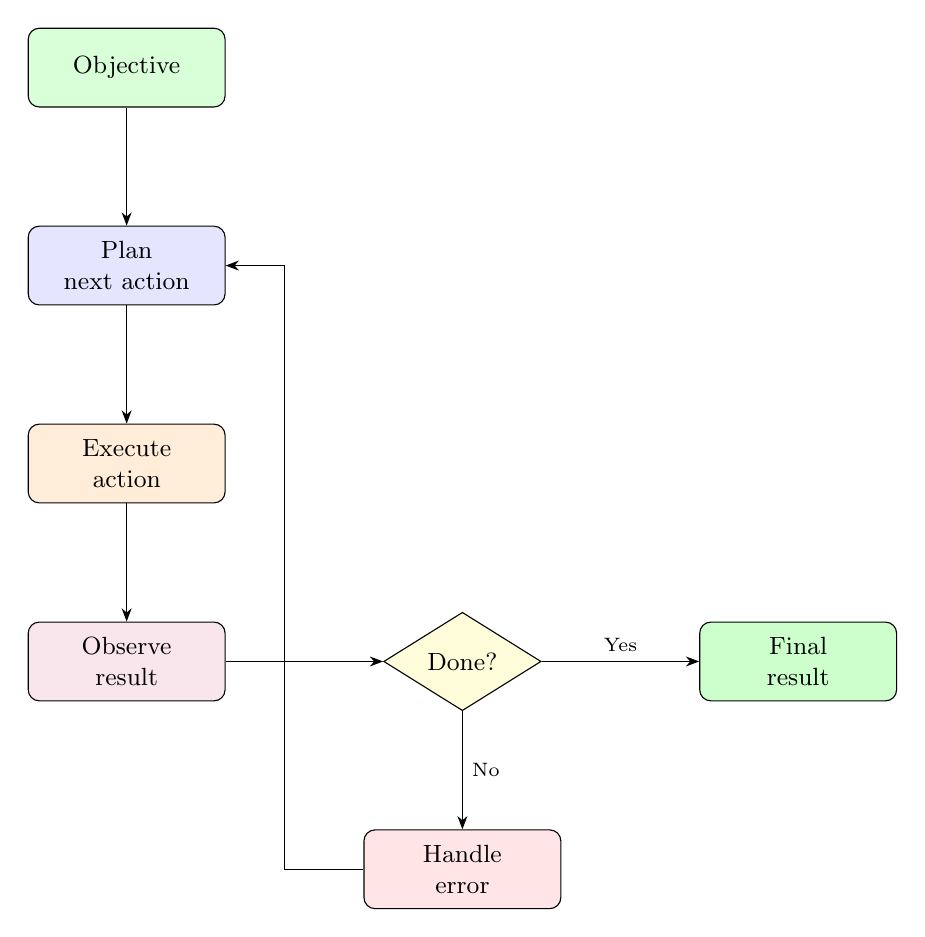
\begin{tikzpicture}[node distance=1.5cm, >=Stealth,
  box/.style={rectangle, rounded corners, draw, fill=#1, minimum height=1cm, minimum width=2.5cm, align=center, font=\small},
  box/.default=blue!10,
  decision/.style={diamond, draw, fill=yellow!15, minimum width=2cm, minimum height=1.2cm, align=center, font=\small, inner sep=1pt}]
  \node[box=green!15] (obj) {Objective};
  \node[box=blue!10, below=of obj] (plan) {Plan\\next action};
  \node[box=orange!15, below=of plan] (act) {Execute\\action};
  \node[box=purple!10, below=of act] (obs) {Observe\\result};
  \node[decision, right=2cm of obs] (done) {Done?};
  \node[box=red!10, below=of done] (error) {Handle\\error};
  \node[box=green!20, right=2cm of done] (success) {Final\\result};
  \draw[->] (obj) -- (plan);
  \draw[->] (plan) -- (act);
  \draw[->] (act) -- (obs);
  \draw[->] (obs) -- (done);
  \draw[->] (done) -- node[right, font=\scriptsize]{No} (error);
  \draw[->] (done) -- node[above, font=\scriptsize]{Yes} (success);
  \draw[->] (error.west) -- ++(-1,0) |- (plan.east);
\end{tikzpicture}
\caption{Agentic AI workflow: decide, act, observe, iterate.}
\label{fig:agent-workflow}
\end{figure}

\section{In Our Project: The Preprocessing Pipeline Agent}

The entire pipeline behaves as an \textbf{orchestration agent}:

\textbf{Objective}: ``Transform raw GitHub data into a validated Knowledge Base, end-to-end, with no human in the loop.''

\textbf{Why this is agentic} (not just a script):
\begin{itemize}
    \item Makes \textbf{decisions}: skip invalid data, rescue borderline cases
    \item Handles \textbf{errors}: API limits, network failures, malformed data
    \item \textbf{Adapts}: new repositories added without code changes
    \item \textbf{Orchestrates}: GitHub API + LLM Vision + similarity engine + schema validator
\end{itemize}

\begin{analogybox}
The Image Agent is a \textbf{specialist} (one task, done autonomously). The Pipeline Agent is a \textbf{project manager}: coordinates sub-processes, handles problems, delivers the final product without asking for help.
\end{analogybox}

% ============================================================
% CHAPTER 14 — VECTOR DATABASES
% ============================================================
\chapter{Vector Databases --- Where Meaning is Stored}

\section{What is a Vector Database?}

A vector database stores embeddings and allows searching by \textbf{meaning} instead of keywords.

\textbf{Traditional DB}: ``Find documents containing the word UART.''

\textbf{Vector DB}: ``Find documents \textit{about} UART problems --- even if they say `serial communication failure'.''

\section{How Vector Search Works}

\begin{enumerate}
    \item All documents → converted to embeddings → stored
    \item User query → converted to an embedding
    \item Database finds the closest stored embeddings (cosine similarity)
    \item Returns top-k most similar documents
\end{enumerate}

\section{The Landscape}

\begin{table}[h]
\centering
\begin{tabularx}{\textwidth}{l l X}
\toprule
\textbf{Database} & \textbf{Type} & \textbf{Used for} \\
\midrule
Azure AI Search & Cloud managed & Our production system \\
ChromaDB & Open source, local & Our local testing \\
Pinecone & Cloud managed & Production RAG \\
FAISS & Library (Meta) & Research, high-performance \\
\bottomrule
\end{tabularx}
\end{table}

\begin{projectbox}
ST ChatGPT uses Azure AI Search as its vector database. We test locally with ChromaDB before uploading.
\end{projectbox}

% ============================================================
% CHAPTER 15 — COMPUTER VISION
% ============================================================
\chapter{Computer Vision --- When AI Sees}

\section{What is Computer Vision?}

Computer Vision enables machines to interpret images and videos --- to ``see'' and extract information from visual content.

\section{Key Tasks}

\begin{table}[h]
\centering
\begin{tabularx}{\textwidth}{l X X}
\toprule
\textbf{Task} & \textbf{What it does} & \textbf{Example} \\
\midrule
Classification & Label an image & ``Circuit diagram'' \\
Object Detection & Locate objects & ``Capacitor at position X,Y'' \\
OCR & Extract text & Read register values from screenshot \\
Image Description & Generate text description & ``Oscilloscope trace at 50MHz'' \\
\bottomrule
\end{tabularx}
\end{table}

\begin{projectbox}
Our Vision Agent uses LLM Vision (Computer Vision + LLM) to describe technical images from STM32 issues, converting visual information into searchable text for RAG.
\end{projectbox}

% ============================================================
% CHAPTER 16 — EVALUATION
% ============================================================
\chapter{Evaluation --- Measuring AI Quality}

\section{Why Evaluation Matters}

``If you cannot measure it, you cannot improve it.'' An AI system without evaluation is a car without a speedometer.

\section{Key Metrics for RAG}

\begin{table}[h]
\centering
\begin{tabularx}{\textwidth}{l X c}
\toprule
\textbf{Metric} & \textbf{What it measures} & \textbf{Perfect} \\
\midrule
P@k & Of top k results, how many are relevant? & 1.0 \\
MRR & How early is the first relevant result? & 1.0 \\
Recall & Of all relevant docs, how many did we find? & 1.0 \\
F1 & Balance of precision and recall & 1.0 \\
Latency & Response speed & $<$ 2s \\
\bottomrule
\end{tabularx}
\end{table}

\section{Offline vs.\ Online Evaluation}

\begin{table}[h]
\centering
\begin{tabularx}{\textwidth}{X X}
\toprule
\textbf{Offline (local)} & \textbf{Online (production)} \\
\midrule
Test on your machine & Test on live platform \\
Fast, repeatable, free & Real conditions \\
Uses TF-IDF / local embeddings & Uses actual RAG engine \\
Catches data quality issues & Catches integration issues \\
\bottomrule
\end{tabularx}
\end{table}

\section{The Iteration Loop}

\begin{enumerate}
    \item Modify pipeline (data, features, chunking)
    \item Regenerate data
    \item Evaluate --- metrics improving?
    \begin{itemize}
        \item YES → Deploy
        \item NO → Back to step 1
    \end{itemize}
\end{enumerate}

\begin{projectbox}
We run offline TF-IDF tests on local JSONs + online 50-question benchmarks on the ST ChatGPT platform.
\end{projectbox}

% ============================================================
% CHAPTER 17 — DATA GENERATION
% ============================================================
\chapter{Data Generation --- Creating New Knowledge}

\section{What is Data Generation?}

Data generation means \textbf{creating new data} that did not previously exist, using algorithms, rules, or AI models.

Unlike data \textit{collection} (gathering what exists), data generation \textbf{produces} new documents from existing information.

\begin{analogybox}
A teacher has 10 exam questions. To make a 100-question practice booklet, they write 90 new questions \textit{inspired by} the originals --- same topics, same difficulty, entirely new text. That's data generation: creating new content from existing knowledge.
\end{analogybox}

\section{Why Generate Data?}

\begin{itemize}
    \item \textbf{Insufficient data}: not enough examples
    \item \textbf{Imbalanced data}: too many of one category
    \item \textbf{Missing structure}: data exists but in unusable form
    \item \textbf{Expensive to collect}: human annotation costs time and money
\end{itemize}

\section{Types of Generated Data}

\begin{table}[h]
\centering
\begin{tabularx}{\textwidth}{l X X}
\toprule
\textbf{Type} & \textbf{Description} & \textbf{Example} \\
\midrule
Synthetic & Created entirely by algorithms & GPT generating fake reviews for testing \\
Augmented & Transformations of existing data & Rotating images for more training samples \\
Derived & Synthesized from multiple sources & Bug reports → troubleshooting guide \\
Simulated & From simulating real scenarios & Virtual sensor data for autonomous driving \\
\bottomrule
\end{tabularx}
\end{table}

\section{Derived Data: The Most Valuable Pattern}

In enterprise AI, \textbf{derived data generation} takes existing structured data and synthesizes \textbf{entirely new documents} that provide more value than the originals:

\begin{itemize}
    \item Multiple bug reports → a \textbf{diagnostic card} (root cause + symptoms + fix)
    \item A long issue thread → a \textbf{resolution guide} (step-by-step)
    \item Raw images → \textbf{text descriptions} (via Vision model)
    \item Individual issues → \textbf{similarity links} between related problems
\end{itemize}

\begin{figure}[h]
\centering
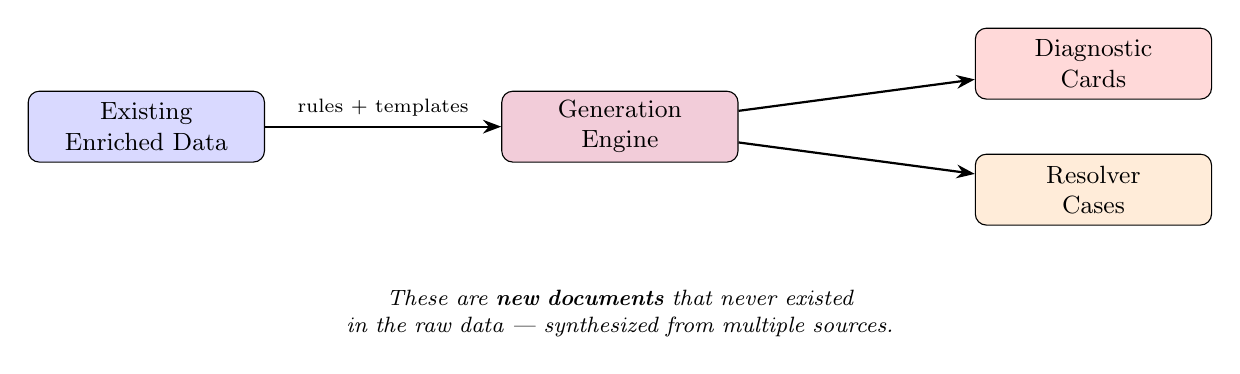
\begin{tikzpicture}[node distance=1.2cm, >=Stealth,
  box/.style={rectangle, rounded corners, draw, fill=#1, minimum height=0.9cm, minimum width=3cm, align=center, font=\small},
  box/.default=blue!10]
  \node[box=blue!15] (source) {Existing\\Enriched Data};
  \node[box=purple!20, right=3cm of source] (engine) {Generation\\Engine};
  \node[box=red!15, right=3cm of engine, yshift=0.8cm] (cards) {Diagnostic\\Cards};
  \node[box=orange!15, right=3cm of engine, yshift=-0.8cm] (cases) {Resolver\\Cases};
  \draw[->, thick] (source) -- node[above, font=\scriptsize]{rules + templates} (engine);
  \draw[->, thick] (engine) -- (cards);
  \draw[->, thick] (engine) -- (cases);
  \node[below=1.5cm of engine, font=\footnotesize\itshape, align=center, text width=8cm] {These are \textbf{new documents} that never existed\\in the raw data --- synthesized from multiple sources.};
\end{tikzpicture}
\caption{Derived data generation: existing data → new knowledge artifacts.}
\label{fig:data-generation}
\end{figure}

\begin{analogybox}
A detective reads 200 witness statements and produces one ``case summary'' with timeline, suspects, and evidence links. The summary is \textit{derived data} --- it didn't exist before, was generated from existing sources, and is more useful than any single statement alone.
\end{analogybox}

\section{Quality Control}

Generated data must be validated:
\begin{itemize}
    \item \textbf{Schema validation}: required fields present?
    \item \textbf{Factual accuracy}: correctly reflects sources?
    \item \textbf{Deduplication}: no redundant artifacts?
    \item \textbf{Usefulness}: can the AI actually retrieve and use it?
\end{itemize}

% ============================================================
% CHAPTER 18 — ADVANTAGES AND LIMITS
% ============================================================
\chapter{Advantages, Limits, and Challenges of AI}

\section{Advantages}

\begin{itemize}
    \item \textbf{Speed}: processes thousands of documents in seconds
    \item \textbf{Consistency}: same input = same processing every time
    \item \textbf{Scalability}: works on any volume once built
    \item \textbf{Pattern discovery}: finds connections humans miss
    \item \textbf{24/7}: never sleeps, never takes breaks
\end{itemize}

\section{Limits}

\begin{itemize}
    \item \textbf{No common sense}: matches patterns, doesn't understand
    \item \textbf{Data dependency}: garbage in = garbage out
    \item \textbf{Hallucination}: generates confident nonsense
    \item \textbf{Bias}: if 90\% of training data is about STM32H7, the model will underperform on STM32F4
    \item \textbf{Explainability}: hard to know WHY a specific answer was generated
    \item \textbf{Cost}: training large models = thousands of GPUs for weeks
\end{itemize}

\section{Ethical Considerations}

\begin{itemize}
    \item \textbf{Privacy}: AI may process sensitive data
    \item \textbf{Fairness}: models must not discriminate
    \item \textbf{Transparency}: users should know they're talking to AI
    \item \textbf{Accountability}: who is responsible when AI is wrong?
\end{itemize}

% ============================================================
% CHAPTER 19 — GLOSSARY
% ============================================================
\chapter{Glossary}

\begin{longtable}{l p{10cm}}
\toprule
\textbf{Term} & \textbf{Definition} \\
\midrule
\endhead
AI & Artificial Intelligence --- systems performing tasks requiring human intelligence \\
ML & Machine Learning --- learning from data instead of explicit rules \\
DL & Deep Learning --- ML with multi-layer neural networks \\
NLP & Natural Language Processing --- AI for understanding text \\
Transformer & Architecture using attention mechanism (basis of all modern LLMs) \\
Attention & Mechanism allowing model to look at all words simultaneously \\
GPT & Generative Pre-trained Transformer \\
Generative AI & AI that creates new content (text, images, code) \\
LLM & Large Language Model --- Transformer trained on massive text \\
RAG & Retrieval-Augmented Generation --- search then answer from your data \\
Embedding & Numerical vector representing the meaning of text \\
Vector DB & Database for searching embeddings by similarity \\
Cosine similarity & Measure of similarity between two vectors (0 to 1) \\
Hallucination & AI generating false information that sounds correct \\
Prompt & Input text sent to an LLM \\
Context window & Maximum text an LLM can process at once \\
Fine-tuning & Additional training on domain-specific data \\
Token & Smallest text unit processed by an LLM \\
Feature Engineering & Extracting structured info from raw data \\
Data Generation & Creating new data from existing sources \\
Agentic AI & AI systems that act autonomously with planning and tools \\
Pipeline & Chain of automated processing steps \\
Knowledge Base (KB) & Document collection feeding a RAG system \\
Chunking & Splitting documents into retrievable pieces \\
TF-IDF & Term Frequency-Inverse Document Frequency \\
P@k & Precision at rank k \\
MRR & Mean Reciprocal Rank \\
Epoch & One complete pass through training data \\
Overfitting & Model memorizes training data, fails on new data \\
Model drift & Model performance degrading over time \\
\bottomrule
\end{longtable}

% ============================================================
% CHAPTER 20 — CONCLUSION
% ============================================================
\chapter{Conclusion}

\section*{The Story in One Page}

This document told a story with a natural progression:

\begin{enumerate}
    \item \textbf{AI} is software that finds patterns --- not magic
    \item \textbf{Machine Learning} taught machines to learn from data instead of rules
    \item \textbf{Deep Learning} made ML powerful enough for language and vision
    \item \textbf{NLP} applied DL to text --- machines started ``reading''
    \item \textbf{Transformers} (attention mechanism) solved NLP's speed and memory problems
    \item \textbf{GPT} was born: a Transformer trained to predict next words became shockingly capable
    \item \textbf{Generative AI} emerged: machines that create text, images, code
    \item \textbf{LLMs} became the engines of modern AI --- but they hallucinate
    \item \textbf{RAG} solved hallucination by grounding LLMs in verified documents
    \item \textbf{Feature Engineering} makes those documents findable
    \item \textbf{Agents} automate the entire workflow end-to-end
    \item \textbf{Data quality drives everything} --- better data = better AI
\end{enumerate}

\section*{The Bottom Line}

AI amplifies human capability. It doesn't replace expertise --- it makes experts faster.

Our project demonstrates this: we don't build the LLM, we don't train the neural network. We \textbf{engineer the data} that makes the AI useful. The chatbot's answer quality depends entirely on the data we provide --- and that's what our pipeline ensures.

\end{document}

\section{What Makes it ``Deep''?}

Deep Learning simply means a neural network with many hidden layers (tens, hundreds, or even thousands). More layers allow the network to learn more complex patterns.

\begin{table}[h]
\centering
\begin{tabularx}{\textwidth}{X X X}
\toprule
\textbf{Simple ML} & \textbf{Shallow Neural Net} & \textbf{Deep Learning} \\
\midrule
Manual feature extraction & 1--2 hidden layers & 10--1000+ hidden layers \\
Works on structured data & Simple pattern recognition & Complex tasks: language, vision, speech \\
\bottomrule
\end{tabularx}
\end{table}

\section{Why Deep Learning Matters}

Deep Learning powers the most impressive AI systems today:
\begin{itemize}
    \item \textbf{Large Language Models} (GPT, Claude, LLaMA) --- text understanding and generation
    \item \textbf{Computer Vision} (image recognition, object detection, face recognition)
    \item \textbf{Speech recognition} (Siri, Alexa, Google Assistant)
    \item \textbf{Machine translation} (Google Translate, DeepL)
\end{itemize}

\begin{projectbox}
The LLM inside ST ChatGPT is a Deep Learning model. We do not train it ourselves --- we feed it our data through RAG.
\end{projectbox}

% ============================================================
% CHAPTER 5 — NLP
% ============================================================
\chapter{Natural Language Processing (NLP)}

\section{What is NLP?}

Natural Language Processing is the branch of AI that enables computers to understand, interpret, and generate human language --- text and speech.

When you type a question to a chatbot and it understands what you mean --- that is NLP at work.

\section{Key NLP Tasks}

\begin{table}[h]
\centering
\begin{tabularx}{\textwidth}{l X X}
\toprule
\textbf{Task} & \textbf{What it does} & \textbf{Example} \\
\midrule
Tokenization & Split text into words/tokens & ``Hello world'' $\rightarrow$ [``Hello'', ``world''] \\
NER & Identify names, places, dates & ``STM32H7 has a DMA bug'' $\rightarrow$ STM32H7=MCU \\
Sentiment Analysis & Detect emotion/opinion & ``This driver works perfectly'' $\rightarrow$ positive \\
Text Classification & Assign categories & Issue $\rightarrow$ bug / feature request / question \\
Summarization & Condense long text & 10-page report $\rightarrow$ 3-sentence summary \\
Question Answering & Find answer in text & ``How to init UART on H7?'' $\rightarrow$ answer \\
\bottomrule
\end{tabularx}
\end{table}

\section{Tokenization in Detail}

Tokenization is the first step of any NLP pipeline. It splits raw text into smaller units (tokens) that the model can process.

\begin{lstlisting}
"HAL_UART_Init() failed on STM32H7"
  -> ["HAL", "_", "UART", "_", "Init", "()", "failed", "on", "STM32", "H7"]
\end{lstlisting}

Modern LLMs use subword tokenization (BPE): common words stay whole, rare words are split into pieces.

\section{TF-IDF: Measuring Word Importance}

TF-IDF (Term Frequency -- Inverse Document Frequency) is a classic NLP technique that measures how important a word is in a document relative to all other documents.

\begin{itemize}
    \item \textbf{TF} (Term Frequency): how often the word appears in THIS document
    \item \textbf{IDF} (Inverse Document Frequency): how rare the word is across ALL documents
    \item \textbf{TF-IDF = TF $\times$ IDF} --- high score means the word is frequent here but rare elsewhere
\end{itemize}

\begin{projectbox}
We use TF-IDF for offline retrieval testing: before uploading to ST ChatGPT, we verify that a simple TF-IDF search on our preprocessed data can find the right documents.
\end{projectbox}

% ============================================================
% CHAPTER 6 — EMBEDDINGS
% ============================================================
\chapter{Embeddings --- How AI Understands Meaning}

\section{The Problem: Computers Only Understand Numbers}

Computers cannot read text the way humans do. They need text to be converted into numbers before they can process it. But not just any numbers --- numbers that capture the MEANING of the text.

\section{What is an Embedding?}

An embedding is a list of numbers (a vector) that represents the meaning of a piece of text. Texts with similar meanings have similar vectors.

``UART initialization error'' and ``USART init failure'' would have very similar embeddings because they mean almost the same thing --- even though the words are different.

\section{How Embeddings are Used}

\begin{itemize}
    \item \textbf{Semantic search}: find documents related to a question based on meaning, not just keywords
    \item \textbf{Similarity detection}: find issues that describe the same bug in different words
    \item \textbf{Clustering}: group related documents together automatically
    \item \textbf{Recommendation}: suggest similar content
\end{itemize}

\section{Cosine Similarity}

Once texts are converted to vectors, we measure how similar they are using cosine similarity --- a number between 0 (completely different) and 1 (identical).

\begin{table}[h]
\centering
\begin{tabularx}{\textwidth}{X X c}
\toprule
\textbf{Text A} & \textbf{Text B} & \textbf{Cosine sim.} \\
\midrule
UART init error on H7 & USART initialization failure STM32H7 & 0.92 \\
UART init error on H7 & How to configure SPI clock & 0.15 \\
\bottomrule
\end{tabularx}
\end{table}

\begin{projectbox}
Our pipeline uses cosine similarity in two places: linking similar issues (similarity stage) and evaluating retrieval quality (benchmark).
\end{projectbox}

% ============================================================
% CHAPTER 7 — LLMs
% ============================================================
\chapter{Large Language Models (LLMs)}

\section{What is an LLM?}

A Large Language Model is a Deep Learning model trained on enormous amounts of text --- books, websites, code, conversations. It learns to predict what word comes next in a sentence, and from this simple task it develops the ability to understand and generate language.

\begin{analogybox}
An LLM is like someone who has read every book, every website, and every forum post in the world. They can talk about anything --- but they might mix things up or make things up if they are not careful.
\end{analogybox}

\section{How LLMs Generate Text}

LLMs generate text one token at a time. For each new token, the model calculates the probability of every possible next word and picks one.

\begin{lstlisting}
Input: "How do I initialize"  -> predicts: "UART"
Then:  "How do I initialize UART"  -> predicts: "on"
Then:  "How do I initialize UART on"  -> predicts: "STM32H7"
...and so on until the full answer is generated
\end{lstlisting}

\section{The Hallucination Problem}

Hallucination is when the AI generates information that sounds correct but is actually false. This is the most dangerous failure mode of any LLM-based system.

\begin{table}[h]
\centering
\begin{tabularx}{\textwidth}{X X}
\toprule
\textbf{Hallucination example} & \textbf{Why it is dangerous} \\
\midrule
``This bug was fixed in version 1.4.2'' & The fix might not exist, leading to wrong firmware choices \\
``Use HAL\_DMA\_Start\_IT() with channel 3'' & Wrong channel could cause hardware damage \\
\bottomrule
\end{tabularx}
\end{table}

\textbf{This is why RAG exists}: by forcing the LLM to answer ONLY from retrieved documents, we dramatically reduce hallucination.

\section{Key LLM Concepts}

\begin{table}[h]
\centering
\begin{tabularx}{\textwidth}{l X}
\toprule
\textbf{Concept} & \textbf{Explanation} \\
\midrule
Prompt & The text you send to the model (question + context + instructions) \\
Context window & Maximum amount of text the model can process at once (e.g.\ 128K tokens) \\
Temperature & Controls randomness: 0 = deterministic, 1 = creative \\
Fine-tuning & Additional training on domain-specific data \\
System prompt & Hidden instructions that define the model's behavior \\
\bottomrule
\end{tabularx}
\end{table}

\begin{projectbox}
ST ChatGPT uses a system prompt (called persona) that defines how the model should behave for STM32 support.
\end{projectbox}

% ============================================================
% CHAPTER 8 — SPECIALIZED CHATBOTS
% ============================================================
\chapter{Specialized Chatbots --- Why and How}

\section{Generalist vs.\ Specialized Chatbot}

\begin{table}[h]
\centering
\begin{tabularx}{\textwidth}{l X X}
\toprule
& \textbf{Generalist chatbot} & \textbf{Specialized chatbot} \\
\midrule
Knowledge & Broad but shallow & Deep in one domain \\
Accuracy & Risk of hallucinations & Answers verified by a KB \\
Example & ChatGPT in free mode & Our STM32 chatbot \\
Data & The entire internet & GitHub issues + STM32 docs \\
\bottomrule
\end{tabularx}
\end{table}

\section{Why Specialize a Chatbot?}

A generalist LLM does NOT know:
\begin{itemize}
    \item The specific bugs of HAL STM32H7 v1.11.0
    \item The exact DMA configuration for an SPI transfer
    \item The workarounds validated by the firmware team
\end{itemize}

$\rightarrow$ You must \textbf{provide the right information at the right time} = that's the role of RAG.

\section{Three Approaches to Specialize a Chatbot}

\begin{table}[h]
\centering
\begin{tabularx}{\textwidth}{l X X X}
\toprule
\textbf{Approach} & \textbf{Principle} & \textbf{Advantages} & \textbf{Disadvantages} \\
\midrule
Fine-tuning & Re-train on your data & Deeply integrated & Expensive, risk of forgetting \\
RAG & Provide docs in context & Flexible, traceable & Depends on retrieval quality \\
Prompt Eng. & Precise instructions & Quick to set up & Limited by context window \\
\bottomrule
\end{tabularx}
\end{table}

\section{Why We Chose RAG}

\begin{itemize}
    \item Our data changes frequently (new issues, new releases)
    \item We need traceability (every answer must cite its source)
    \item Fine-tuning would require re-training every time data changes = too expensive
    \item RAG lets us update the knowledge base in minutes without touching the model
\end{itemize}

\begin{projectbox}
We use RAG because our technical data evolves constantly (new issues, new firmware releases). Our pipeline focuses on producing high-quality, well-structured data so the RAG retrieval finds the right documents when users ask questions.
\end{projectbox}

% ============================================================
% CHAPTER 9 — RAG
% ============================================================
\chapter{RAG --- Retrieval-Augmented Generation}

\section{The Problem RAG Solves}

Standard LLMs answer from their training data --- which is frozen at a point in time, generic, and may contain errors.

\begin{table}[h]
\centering
\begin{tabularx}{\textwidth}{X X}
\toprule
\textbf{Standard LLM} & \textbf{LLM with RAG} \\
\midrule
Answers from general training data & Answers from YOUR specific documents \\
May be outdated & Uses latest uploaded data \\
Cannot cite sources & Every answer traces back to a source \\
Higher hallucination risk & Hallucination reduced by grounding \\
\bottomrule
\end{tabularx}
\end{table}

\section{How RAG Works --- Step by Step}

\begin{enumerate}
    \item \textbf{User asks a question} --- e.g.\ ``How to configure DMA on STM32H7?''
    \item \textbf{RETRIEVAL} --- The system searches the Knowledge Base for the most similar documents (using embeddings + cosine similarity)
    \item \textbf{Top-k documents retrieved} --- The most relevant chunks are selected
    \item \textbf{AUGMENTED GENERATION} --- The LLM receives: user question + retrieved documents
    \item \textbf{Answer generated} --- The LLM synthesizes a precise, sourced answer from those documents
\end{enumerate}

\textbf{In summary}: RAG = ``Search first in the knowledge base, then give the LLM the right documents so it generates a precise answer.''

\begin{figure}[h]
\centering
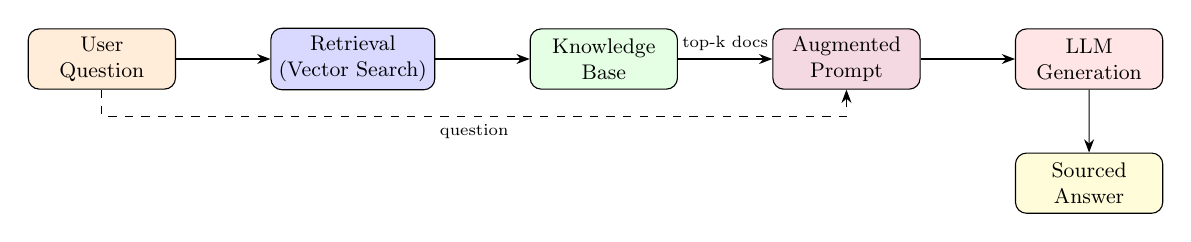
\begin{tikzpicture}[node distance=1.2cm, >=Stealth, scale=0.85, every node/.style={scale=0.85},
  box/.style={rectangle, rounded corners, draw, fill=#1, minimum height=0.9cm, minimum width=2.2cm, align=center, font=\small},
  box/.default=blue!10]
  \node[box=orange!15] (user) {User\\Question};
  \node[box=blue!15, right=of user] (retrieval) {Retrieval\\(Vector Search)};
  \node[box=green!10, right=of retrieval] (kb) {Knowledge\\Base};
  \node[box=purple!15, right=of kb] (augment) {Augmented\\Prompt};
  \node[box=red!10, right=of augment] (llm) {LLM\\Generation};
  \node[box=yellow!15, below=0.8cm of llm] (answer) {Sourced\\Answer};
  \draw[->] (user) -- (retrieval);
  \draw[->] (retrieval) -- (kb);
  \draw[->] (kb) -- node[above, font=\scriptsize]{top-k docs} (augment);
  \draw[->] (augment) -- (llm);
  \draw[->] (llm) -- (answer);
  \draw[->, dashed] (user.south) -- ++(0,-0.4) -| node[below, pos=0.25, font=\scriptsize]{question} (augment.south);
\end{tikzpicture}
\caption{How RAG answers a user question: Retrieval $\rightarrow$ Augmentation $\rightarrow$ Generation.}
\label{fig:rag-flow}
\end{figure}

\section{Why Data Quality is CRITICAL for RAG}

The RAG can only answer correctly if:
\begin{enumerate}
    \item \textbf{The right data exists} in the Knowledge Base (Data Generation)
    \item \textbf{The data is well structured} to be found (Feature Engineering + Chunking)
    \item \textbf{The retrieval finds the right documents} (Similarity + Evaluation)
\end{enumerate}

$\rightarrow$ \textbf{This is exactly the role of our pipeline}: transform raw data into optimized data so that RAG works well.

\begin{figure}[h]
\centering
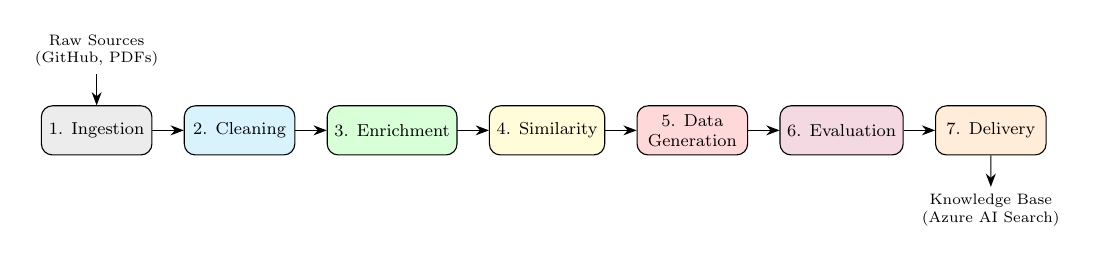
\begin{tikzpicture}[node distance=0.4cm, >=Stealth, scale=0.78, every node/.style={scale=0.78},
  stage/.style={rectangle, rounded corners, draw, fill=#1, minimum height=0.8cm, minimum width=1.8cm, align=center, font=\footnotesize},
  stage/.default=blue!10]
  \node[stage=gray!15] (ingest) {1. Ingestion};
  \node[stage=cyan!15, right=of ingest] (clean) {2. Cleaning};
  \node[stage=green!15, right=of clean] (enrich) {3. Enrichment};
  \node[stage=yellow!15, right=of enrich] (sim) {4. Similarity};
  \node[stage=red!15, right=of sim] (gen) {5. Data\\Generation};
  \node[stage=purple!15, right=of gen] (eval) {6. Evaluation};
  \node[stage=orange!15, right=of eval] (deliv) {7. Delivery};
  \draw[->] (ingest) -- (clean);
  \draw[->] (clean) -- (enrich);
  \draw[->] (enrich) -- (sim);
  \draw[->] (sim) -- (gen);
  \draw[->] (gen) -- (eval);
  \draw[->] (eval) -- (deliv);
  \node[above=0.4cm of ingest, font=\scriptsize, align=center] (src) {Raw Sources\\(GitHub, PDFs)};
  \draw[->] (src) -- (ingest);
  \node[below=0.4cm of deliv, font=\scriptsize, align=center] (kb) {Knowledge Base\\(Azure AI Search)};
  \draw[->] (deliv) -- (kb);
\end{tikzpicture}
\caption{End-to-end pipeline architecture: from raw data sources to RAG-ready Knowledge Base.}
\label{fig:pipeline-architecture}
\end{figure}
\end{tikzpicture}
\caption{End-to-end pipeline architecture: from raw data sources to RAG-ready Knowledge Base.}
\label{fig:pipeline-architecture}
\end{figure}

\section{Chunking Strategies for RAG}

\begin{table}[h]
\centering
\begin{tabularx}{\textwidth}{l X X}
\toprule
\textbf{Strategy} & \textbf{How it works} & \textbf{Pros / Cons} \\
\midrule
Full document & 1 chunk = entire document & Simple but noisy for large docs \\
Paragraph & Split on paragraph boundaries & Clean, preserves meaning \\
Sliding window & Fixed-size with overlap & Uniform size, but cuts meaning \\
Section-based & Split on headers & Great for structured docs \\
Parent-child & Children for search, parents for context & Best for generation quality \\
\bottomrule
\end{tabularx}
\end{table}

\begin{projectbox}
ST ChatGPT uses the parent-child strategy. Our preprocessing pipeline is entirely designed to produce data that works well with this strategy.
\end{projectbox}

% ============================================================
% CHAPTER 10 — FEATURE ENGINEERING
% ============================================================
\chapter{Feature Engineering --- The Secret Sauce}

\section{What is Feature Engineering?}

Feature Engineering is the art of \textbf{extracting and creating structured information} from raw data to help an AI system work better.

\begin{analogybox}
You have a pile of 5,000 paper CVs. Feature Engineering = reading each CV and filling an Excel spreadsheet with columns: ``Years of experience'', ``Main language'', ``Industry sector'', ``Education level''. This structured table is far more exploitable than the raw CVs.
\end{analogybox}

\section{Why It's the Most Impactful Step}

In any AI/ML project, feature engineering typically delivers more improvement than changing algorithms. A simple algorithm with great features outperforms a complex algorithm with poor features.

\begin{lstlisting}
Raw text: "HAL_SPI_Transmit returns HAL_TIMEOUT on NUCLEO-H743ZI 
           when DMA is used with buffer size > 65535 bytes"

Feature Engineering extracts:
  layer = "HAL"              (detected from HAL_ prefix)
  component = "SPI"          (detected from function name)
  board = "NUCLEO-H743ZI"   (detected from pattern)
  severity = "high"          (timeout = functional failure)
  issue_kind = "bug_report"  (labeled as bug)
  keywords = ["DMA", "buffer size", "65535", "timeout"]
  evidence_strength = "high" (specific, reproducible)
\end{lstlisting}

\section{Concrete Examples in Our Project}

\begin{table}[h]
\centering
\begin{tabularx}{\textwidth}{X X X X}
\toprule
\textbf{Raw data} & \textbf{Feature} & \textbf{How} & \textbf{Utility for RAG} \\
\midrule
``HAL\_SPI\_Transmit returns HAL\_TIMEOUT'' & layer = ``HAL'' & Pattern ``HAL\_'' & Filter by layer \\
Labels: [``bug'', ``STM32H7''] & severity = ``high'' & Label mapping & Prioritization \\
Issue with 12 comments & evidence = ``high'' & Richness score & Prioritize rich content \\
Attached image & image\_description & LLM Vision & Make image searchable \\
\bottomrule
\end{tabularx}
\end{table}

\section{Why It's Critical for RAG}

Without feature engineering: RAG searches in raw unstructured text $\rightarrow$ mediocre results.

With feature engineering: RAG can filter, weight, and target $\rightarrow$ relevant results.

\begin{projectbox}
Our enrichment stage performs heavy feature engineering --- extracting layer, severity, board, component, issue\_kind, keywords, and evidence strength from every issue and file.
\end{projectbox}

% ============================================================
% CHAPTER 11 — AGENTIC AI
% ============================================================
\chapter{Agentic AI --- Autonomous Intelligent Agents}

\section{What is an AI Agent?}

An \textbf{AI agent} is an autonomous program that:
\begin{enumerate}
    \item \textbf{Receives an objective} (not just a simple instruction)
    \item \textbf{Plans} the steps to achieve that objective
    \item \textbf{Executes} actions (call APIs, read files, make decisions)
    \item \textbf{Observes} the results
    \item \textbf{Adapts} if something fails (retries, alternative plan)
\end{enumerate}

\textbf{The key difference with a simple LLM call:}

\begin{lstlisting}
Simple LLM call:   Question -> Answer (one shot)
Agentic AI:        Objective -> Planning -> Action 1 -> Observation 
                   -> Action 2 -> ... -> Final result
\end{lstlisting}

\section{Analogy}

\begin{analogybox}
\textbf{Simple LLM} = A consultant you ask ONE question and they answer.

\textbf{AI Agent} = An autonomous intern given ONE mission. They plan their steps, execute, handle problems, and come back with the final result.
\end{analogybox}

\section{Components of an AI Agent}

\begin{itemize}
    \item \textbf{LLM (brain)}: reasoning and decision-making
    \item \textbf{Tools}: APIs, file access, databases, web search
    \item \textbf{Memory}: context of past actions and observations
    \item \textbf{Execution loop}: Plan $\rightarrow$ Act $\rightarrow$ Observe $\rightarrow$ Adapt $\rightarrow$ Repeat until done
\end{itemize}

\section{Types of AI Agents}

\begin{table}[h]
\centering
\begin{tabularx}{\textwidth}{l X X}
\toprule
\textbf{Type} & \textbf{Behavior} & \textbf{Example} \\
\midrule
Reactive & Responds to stimuli, no planning & Simple chatbot with if/else \\
Deliberative & Plans before acting & Our image enrichment agent \\
Multi-agent & Several agents collaborate & One collects data, another evaluates \\
\bottomrule
\end{tabularx}
\end{table}

\section{In Our Project: The Image Enrichment Agent}

\textbf{Objective given to the agent}: ``For each GitHub issue containing images, generate a textual description of each image.''

\textbf{What the agent does autonomously}:
\begin{enumerate}
    \item Scans all issues with images
    \item Extracts image URLs
    \item Calls the LLM Vision API to analyze each image
    \item If an image is inaccessible $\rightarrow$ handles the error, moves to the next
    \item If the API rate limit is hit $\rightarrow$ waits and retries
    \item Inserts the generated description into the correct document field
    \item Verifies coherence of the final result
\end{enumerate}

$\rightarrow$ \textbf{Autonomy + error handling + orchestration} = that's Agentic AI.

\begin{figure}[h]
\centering
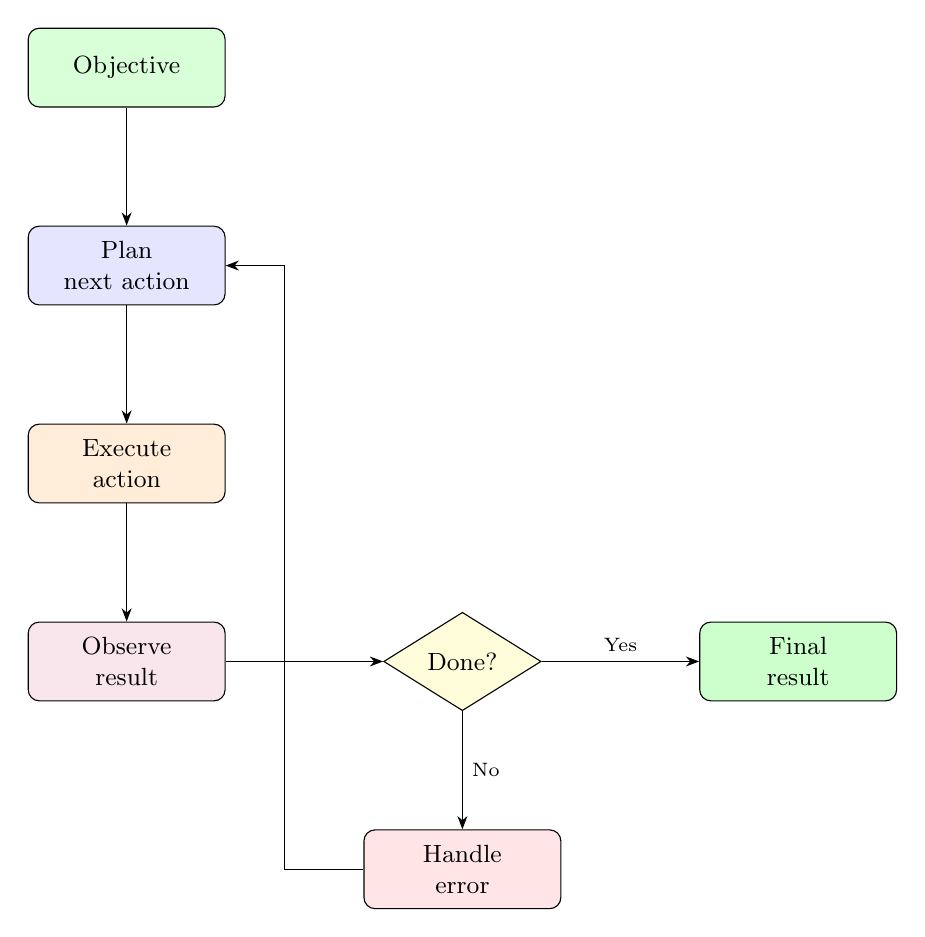
\begin{tikzpicture}[node distance=1.5cm, >=Stealth,
  box/.style={rectangle, rounded corners, draw, fill=#1, minimum height=1cm, minimum width=2.5cm, align=center, font=\small},
  box/.default=blue!10,
  decision/.style={diamond, draw, fill=yellow!15, minimum width=2cm, minimum height=1.2cm, align=center, font=\small, inner sep=1pt}]
  \node[box=green!15] (obj) {Objective};
  \node[box=blue!10, below=of obj] (plan) {Plan\\next action};
  \node[box=orange!15, below=of plan] (act) {Execute\\action};
  \node[box=purple!10, below=of act] (obs) {Observe\\result};
  \node[decision, right=2cm of obs] (done) {Done?};
  \node[box=red!10, below=of done] (error) {Handle\\error};
  \node[box=green!20, right=2cm of done] (success) {Final\\result};
  \draw[->] (obj) -- (plan);
  \draw[->] (plan) -- (act);
  \draw[->] (act) -- (obs);
  \draw[->] (obs) -- (done);
  \draw[->] (done) -- node[right, font=\scriptsize]{No} (error);
  \draw[->] (done) -- node[above, font=\scriptsize]{Yes} (success);
  \draw[->] (error.west) -- ++(-1,0) |- (plan.east);
\end{tikzpicture}
\caption{Agentic AI workflow: the agent autonomously decides, acts, observes, and iterates.}
\label{fig:agent-workflow}
\end{figure}

\section{Why Agentic AI Matters for Industry}

AI Agents allow \textbf{automating complex workflows} that previously required human intervention at every step:
\begin{itemize}
    \item Process automation at scale (thousands of documents)
    \item Intelligent data pipelines
    \item Self-healing systems that detect and fix issues
    \item Multi-step research and analysis tasks
\end{itemize}

\begin{projectbox}
Our Vision agent enriches thousands of images autonomously, handling errors, retries, and incremental updates without manual intervention.
\end{projectbox}

\section{In Our Project: The Preprocessing Agent}

Beyond image enrichment, the entire preprocessing pipeline itself behaves as an \textbf{orchestration agent}:

\textbf{Objective given to the agent}: ``Transform raw GitHub data into a complete, validated Knowledge Base --- end to end, with no human in the loop.''

\textbf{What the agent does autonomously}:
\begin{enumerate}
    \item Detects which repositories have new data (ingestion trigger)
    \item Fetches new issues, PRs, commits, and files via GitHub API
    \item Cleans, normalizes, and filters invalid content
    \item Enriches each document with metadata (layer, severity, board, component)
    \item Computes similarity links between related issues
    \item Generates new artifacts (diagnostic cards, resolver cases)
    \item Runs evaluation benchmarks to verify quality
    \item Packages and delivers to the Knowledge Base
    \item If a step fails $\rightarrow$ logs the error, skips the problematic item, continues
\end{enumerate}

\textbf{Why this is agentic} (not just a script):
\begin{itemize}
    \item It makes \textbf{decisions}: skip invalid data, rescue borderline cases, choose chunking strategy
    \item It handles \textbf{errors}: API rate limits, network failures, malformed data
    \item It \textbf{adapts}: new repositories can be added without changing the logic
    \item It \textbf{orchestrates} multiple tools: GitHub API, LLM Vision, similarity engine, schema validator
\end{itemize}

\begin{analogybox}
If the Image Agent is a specialist (one task, done autonomously), the Preprocessing Agent is a project manager: it coordinates an entire team of sub-processes, makes decisions when things go wrong, and delivers the final product without asking for help.
\end{analogybox}

% ============================================================
% CHAPTER 12 — VECTOR DATABASES
% ============================================================
\chapter{Vector Databases}

\section{What is a Vector Database?}

A vector database is a specialized storage system designed to store and search embeddings efficiently. Instead of searching by keywords (like a traditional database), it searches by meaning (similarity).

\textbf{Traditional database}: ``Find all documents containing the word UART.''

\textbf{Vector database}: ``Find all documents that are ABOUT UART problems, even if they use different words.''

\section{How Vector Search Works}

\begin{enumerate}
    \item All documents are converted to embeddings and stored
    \item When a query arrives, it is also converted to an embedding
    \item The database finds the stored embeddings closest to the query embedding
    \item Returns the top-k most similar documents
\end{enumerate}

\section{Popular Vector Databases}

\begin{table}[h]
\centering
\begin{tabularx}{\textwidth}{l l X}
\toprule
\textbf{Database} & \textbf{Type} & \textbf{Used for} \\
\midrule
ChromaDB & Open source, local & Prototyping, local experiments \\
Pinecone & Cloud managed & Production RAG systems \\
Weaviate & Open source, cloud/local & Enterprise applications \\
FAISS & Facebook library & Research, high-performance search \\
\bottomrule
\end{tabularx}
\end{table}

\begin{projectbox}
Our RAG benchmark uses ChromaDB locally for prototyping and testing. The ST ChatGPT production platform uses Azure AI Search as its vector database for storing and retrieving document embeddings at scale.
\end{projectbox}

% ============================================================
% CHAPTER 13 — COMPUTER VISION
% ============================================================
\chapter{Computer Vision}

\section{What is Computer Vision?}

Computer Vision is the field of AI that enables machines to interpret and understand images and videos. It allows computers to ``see'' and extract information from visual content.

\section{Key Computer Vision Tasks}

\begin{table}[h]
\centering
\begin{tabularx}{\textwidth}{l X X}
\toprule
\textbf{Task} & \textbf{What it does} & \textbf{Example} \\
\midrule
Image Classification & Assign a label to an image & ``This is a circuit diagram'' \\
Object Detection & Find and locate objects & ``Capacitor at position X,Y'' \\
OCR & Extract text from images & Read register values from screenshot \\
Image Segmentation & Identify every pixel's category & Separate foreground from background \\
Image Description & Generate text describing content & ``Oscilloscope trace at 50MHz'' \\
\bottomrule
\end{tabularx}
\end{table}

\begin{projectbox}
Our Vision Agent uses Computer Vision (via LLM Vision) to describe technical images extracted from STM32Cube issues, converting visual information into searchable text for RAG.
\end{projectbox}

% ============================================================
% CHAPTER 14 — EVALUATION
% ============================================================
\chapter{Evaluation --- How We Measure AI Quality}

\section{Why Evaluation Matters}

``If you cannot measure it, you cannot improve it.'' --- Lord Kelvin

An AI system without evaluation is like a car without a speedometer --- you have no idea if it is working correctly.

\section{Key Metrics for RAG Systems}

\begin{table}[h]
\centering
\begin{tabularx}{\textwidth}{l X c}
\toprule
\textbf{Metric} & \textbf{What it measures} & \textbf{Good score} \\
\midrule
P@k & Of top k retrieved docs, how many are relevant? & 1.0 \\
MRR & How early does the first relevant doc appear? & 1.0 \\
Recall & Of all relevant docs, how many did we find? & 1.0 \\
F1 Score & Balance between precision and recall & $\rightarrow$ 1.0 \\
Latency & How fast the system responds & $<$ 2s \\
\bottomrule
\end{tabularx}
\end{table}

\section{Offline vs.\ Online Evaluation}

\begin{table}[h]
\centering
\begin{tabularx}{\textwidth}{X X}
\toprule
\textbf{Offline evaluation} & \textbf{Online evaluation} \\
\midrule
Test on your local machine & Test on the live platform \\
Fast, repeatable, no cost & Real conditions, real model \\
Uses TF-IDF, local embeddings & Uses the actual RAG engine \\
Catches data quality issues & Catches integration issues \\
\bottomrule
\end{tabularx}
\end{table}

\section{The Data-Driven Iteration Loop}

\begin{enumerate}
    \item \textbf{Modify} the pipeline (data, features, chunking)
    \item \textbf{Regenerate} the data
    \item \textbf{Evaluate} --- are metrics improving?
    \begin{itemize}
        \item YES $\rightarrow$ Deploy
        \item NO $\rightarrow$ Go back to step 1
    \end{itemize}
    \item \textbf{Measure impact} on production chatbot
\end{enumerate}

\begin{projectbox}
We run both: offline TF-IDF tests on chunked JSONs + online 30Q/50Q benchmarks on the ST ChatGPT platform.
\end{projectbox}

% ============================================================
% CHAPTER 15 — DATA GENERATION
% ============================================================
\chapter{Data Generation --- Synthetic and Derived Data}

\section{What is Data Generation?}

In AI, \textbf{data generation} (also called \textit{synthetic data generation}) refers to the process of \textbf{creating new data} that did not previously exist, using algorithms, rules, or other AI models.

Unlike data \textit{collection} (gathering existing data from the real world), data generation \textbf{produces} new examples, documents, or knowledge artifacts --- often from existing data that serves as a seed.

\begin{analogybox}
Imagine a teacher who has 10 exam questions. To make a practice booklet with 100 questions, the teacher writes 90 new questions \textit{inspired by} the original 10 --- same topics, same difficulty, but entirely new text. That is data generation: creating new content from existing knowledge.
\end{analogybox}

\section{Why Generate Data?}

AI systems are hungry for data. But real-world data is often:

\begin{itemize}
    \item \textbf{Insufficient} --- not enough examples to train or evaluate a model
    \item \textbf{Imbalanced} --- too many examples of one category, too few of another
    \item \textbf{Unstructured} --- exists in a raw form that AI cannot directly use
    \item \textbf{Incomplete} --- missing labels, metadata, or relationships
    \item \textbf{Expensive to collect} --- requires human annotation (time + cost)
\end{itemize}

Data generation solves these problems by \textbf{creating what is missing} rather than waiting to find it in the real world.

\section{Types of Data Generation}

\begin{table}[h]
\centering
\begin{tabularx}{\textwidth}{l X X}
\toprule
\textbf{Type} & \textbf{Description} & \textbf{Example} \\
\midrule
Synthetic data & Created entirely by algorithms or models & GPT generating fake customer reviews for testing \\
Augmented data & Transformations of existing data & Rotating/flipping images to create more training samples \\
Derived data & New documents synthesized from multiple sources & Combining a bug report + its fix into a troubleshooting guide \\
Simulated data & Generated by simulating real-world scenarios & Virtual sensor readings for autonomous driving \\
\bottomrule
\end{tabularx}
\end{table}

\section{Techniques for Generating Data}

\subsection{Rule-Based Generation}

Using predefined rules and templates to produce structured outputs from raw inputs.

\begin{itemize}
    \item A script reads 5 related bug reports and generates a single ``troubleshooting card'' combining their symptoms and solutions
    \item Template-based generation: fill-in-the-blank structures populated with extracted facts
\end{itemize}

\subsection{Model-Based Generation}

Using AI models (often LLMs) to generate new data:

\begin{itemize}
    \item \textbf{Paraphrasing} --- rewriting existing text in different ways to create training variety
    \item \textbf{Summarization} --- condensing long documents into structured knowledge cards
    \item \textbf{Question generation} --- creating Q\&A pairs from documentation for RAG evaluation
    \item \textbf{Image captioning} --- using vision models to produce textual descriptions of images
\end{itemize}

\subsection{Data Augmentation (for Deep Learning)}

Transforming existing samples to create more training data:

\begin{itemize}
    \item \textbf{Images}: rotation, cropping, color changes, adding noise
    \item \textbf{Text}: synonym replacement, back-translation, random insertion/deletion
    \item \textbf{Audio}: speed change, pitch shift, background noise addition
\end{itemize}

\begin{analogybox}
Data augmentation is like a photographer taking the same subject from 20 different angles. The subject is the same, but each photo teaches the model something slightly different about it.
\end{analogybox}

\section{Data Generation vs. Data Collection}

\begin{table}[h]
\centering
\begin{tabularx}{\textwidth}{X X}
\toprule
\textbf{Data Collection} & \textbf{Data Generation} \\
\midrule
Gathers existing real-world data & Creates new data that did not exist before \\
Limited by what already exists & Can produce unlimited quantities \\
Expensive (human labeling, surveys) & Cheap once the generator is built \\
Guaranteed to be realistic & Must be validated for quality \\
May have privacy constraints & No privacy issues (synthetic) \\
\bottomrule
\end{tabularx}
\end{table}

\section{Derived Data: From Existing Knowledge to New Artifacts}

A particularly important pattern in enterprise AI is \textbf{derived data generation}: taking existing structured data and \textbf{synthesizing entirely new documents} that provide value beyond the originals.

Examples:
\begin{itemize}
    \item Multiple related bug reports $\rightarrow$ a single \textbf{diagnostic card} (root cause + symptoms + fix)
    \item A long issue thread with a confirmed solution $\rightarrow$ a \textbf{resolution guide} (step-by-step instructions)
    \item Raw images embedded in documents $\rightarrow$ \textbf{textual descriptions} (generated by a vision model)
    \item Individual data points $\rightarrow$ \textbf{similarity links} connecting related items
\end{itemize}

The key distinction: derived data is \textbf{not a copy} of the source --- it is a new, structured artifact that \textbf{adds value} by combining, summarizing, or restructuring information from multiple sources.

\begin{figure}[h]
\centering
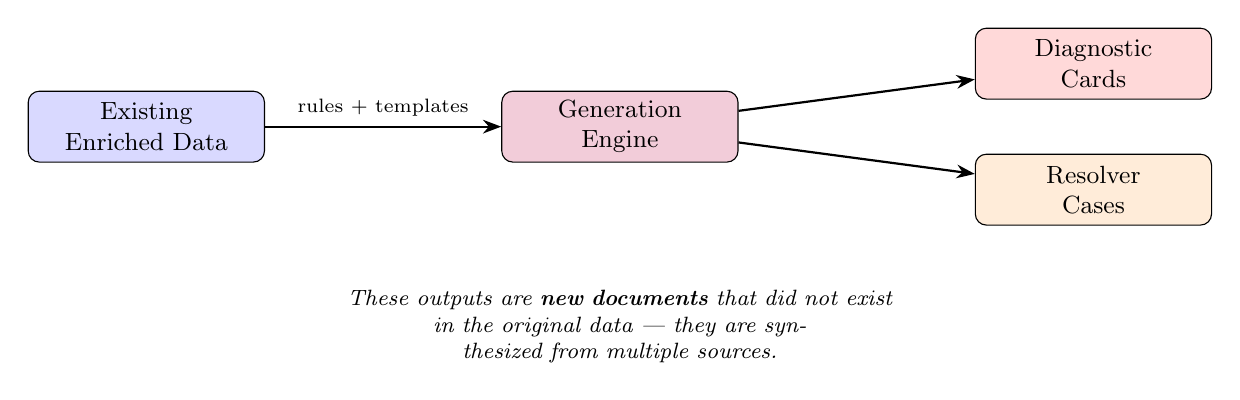
\begin{tikzpicture}[node distance=1.2cm, >=Stealth,
  box/.style={rectangle, rounded corners, draw, fill=#1, minimum height=0.9cm, minimum width=3cm, align=center, font=\small},
  box/.default=blue!10]
  \node[box=blue!15] (source) {Existing\\Enriched Data};
  \node[box=purple!20, right=3cm of source] (engine) {Generation\\Engine};
  \node[box=red!15, right=3cm of engine, yshift=0.8cm] (cards) {Diagnostic\\Cards};
  \node[box=orange!15, right=3cm of engine, yshift=-0.8cm] (cases) {Resolver\\Cases};
  \draw[->, thick] (source) -- node[above, font=\scriptsize]{rules + templates} (engine);
  \draw[->, thick] (engine) -- (cards);
  \draw[->, thick] (engine) -- (cases);
  % Annotation
  \node[below=1.5cm of engine, font=\footnotesize\itshape, align=center, text width=8cm] {These outputs are \textbf{new documents} that did not exist\\in the original data --- they are synthesized from multiple sources.};
\end{tikzpicture}
\caption{Derived data generation: existing enriched data is transformed into entirely new knowledge artifacts.}
\label{fig:data-generation}
\end{figure}

\begin{analogybox}
Think of a detective who reads 200 witness statements and produces a single ``case summary'' with timeline, suspects, and evidence links. That summary is \textit{derived data} --- it did not exist before, but it was generated from existing sources and is more useful than any single statement alone.
\end{analogybox}

\section{Quality Control in Data Generation}

Generated data must be validated:

\begin{itemize}
    \item \textbf{Schema validation} --- does the generated document have all required fields?
    \item \textbf{Factual accuracy} --- does it correctly reflect the source data?
    \item \textbf{Deduplication} --- are we generating redundant artifacts?
    \item \textbf{Usefulness testing} --- can the generated data actually be retrieved and used by the AI system?
\end{itemize}

Without quality control, generated data can introduce \textbf{noise} or \textbf{hallucinated facts} into the system.

\section{Key Takeaways}

\begin{itemize}
    \item Data generation = creating \textbf{new data} (not just collecting existing data)
    \item It solves problems of data scarcity, imbalance, and structure
    \item Techniques range from simple rules to advanced LLM-based synthesis
    \item \textbf{Derived data} transforms existing information into more valuable, structured artifacts
    \item Quality validation is essential to avoid propagating errors
\end{itemize}

% ============================================================
% CHAPTER 16 — ADVANTAGES AND LIMITS
% ============================================================
\chapter{Advantages, Limits, and Challenges of AI}

\section{Advantages}

\begin{itemize}
    \item \textbf{Speed}: processes thousands of documents in seconds
    \item \textbf{Consistency}: same input always gets the same processing
    \item \textbf{Scalability}: once built, works on any volume of data
    \item \textbf{Pattern discovery}: finds connections humans might miss
    \item \textbf{24/7 availability}: works anytime without breaks
\end{itemize}

\section{Limits}

\begin{itemize}
    \item \textbf{No common sense}: AI does not truly understand --- it matches patterns
    \item \textbf{Data dependency}: garbage in = garbage out
    \item \textbf{Hallucination}: can generate confident but wrong answers
    \item \textbf{Bias}: if the training data contains unbalanced or prejudiced information (e.g.\ more examples from one category than another), the AI will reproduce and amplify those imbalances in its outputs. Example: if 90\% of training issues are about STM32H7, the chatbot will perform poorly on STM32F4 questions.
    \item \textbf{Explainability}: hard to know WHY the model gave a specific answer (the internal reasoning is opaque)
    \item \textbf{Cost}: training large models requires massive compute resources (thousands of GPUs for weeks)
\end{itemize}

\section{Ethical Considerations}

\begin{itemize}
    \item \textbf{Privacy}: AI systems may process sensitive data
    \item \textbf{Fairness}: models must not discriminate
    \item \textbf{Transparency}: users should know when they are interacting with AI
    \item \textbf{Accountability}: who is responsible when AI makes a mistake?
\end{itemize}

AI is a tool. Like any tool, its impact depends on how responsibly it is designed, deployed, and monitored.

% ============================================================
% CHAPTER 17 — GLOSSARY
% ============================================================
\chapter{Glossary}

\begin{longtable}{l p{10cm}}
\toprule
\textbf{Term} & \textbf{Definition} \\
\midrule
\endhead
AI & Artificial Intelligence --- systems that perform tasks requiring human intelligence \\
ML & Machine Learning --- learning from data instead of explicit rules \\
DL & Deep Learning --- ML with multi-layer neural networks \\
NLP & Natural Language Processing --- AI for understanding text and speech \\
LLM & Large Language Model --- AI trained on massive text data \\
RAG & Retrieval-Augmented Generation --- search then answer from your own data \\
Embedding & Numerical representation of text that captures meaning \\
Chunking & Splitting documents into smaller pieces for processing \\
Vector DB & Database optimized for searching embeddings by similarity \\
TF-IDF & Term Frequency-Inverse Document Frequency --- measures word importance \\
Cosine similarity & Mathematical measure of similarity between two vectors (0 to 1) \\
Hallucination & When AI generates false information that sounds correct \\
Prompt & The input text sent to an LLM (question + context + instructions) \\
Fine-tuning & Additional training of a model on domain-specific data \\
Token & Smallest unit of text processed by an LLM \\
P@k & Precision at rank k --- fraction of top-k results that are relevant \\
MRR & Mean Reciprocal Rank --- how early the first relevant result appears \\
Feature Engineering & Extracting structured information from raw data \\
Data Generation & Creating structured data from raw unstructured sources \\
Agentic AI & AI systems that act autonomously --- plan, execute, observe, adapt \\
AI Agent & Autonomous program that pursues objectives using tools and reasoning \\
CI/CD & Continuous Integration / Continuous Deployment \\
Pipeline & Chain of automated processing steps executed sequentially \\
Knowledge Base (KB) & Structured collection of documents feeding a RAG system \\
Black box & System whose internal workings are not visible \\
Reverse engineering & Studying a system's behavior to understand its internal logic \\
\bottomrule
\end{longtable}

% ============================================================
% CHAPTER 19 — CONCLUSION
% ============================================================
\chapter{Conclusion}

\section*{Key Takeaways}

\begin{itemize}
    \item \textbf{AI is not magic} --- it is software built on mathematics and data
    \item \textbf{Machine Learning} lets systems learn from examples instead of explicit rules
    \item \textbf{Deep Learning} enables complex tasks like language understanding and image recognition
    \item \textbf{NLP} is what allows AI to understand and generate human text
    \item \textbf{LLMs} are powerful but can hallucinate --- they need guardrails
    \item \textbf{RAG} solves hallucination by grounding answers in your own documents
    \item \textbf{Feature Engineering} is often more impactful than the algorithm itself
    \item \textbf{Agentic AI} enables autonomous, multi-step workflows at scale
    \item \textbf{Data Generation} transforms raw chaos into structured knowledge
    \item \textbf{Evaluation} is not optional --- you must measure to improve
    \item \textbf{CI/CD} enables continuous improvement without manual effort
    \item \textbf{Data quality drives everything} --- better data = better AI
\end{itemize}

\section*{The Bottom Line}

AI is a tool that amplifies human capability. It does not replace expertise --- it makes experts faster and more effective.

Our project demonstrates this: we don't build the LLM, we don't train the neural network. We \textbf{engineer the data} that makes the AI useful. The quality of the chatbot's answers depends entirely on the quality of the data we provide --- and that's what our pipeline ensures.

\end{document}
